% HealthScore Research Manuscript — Camera-Ready Copy (CRC) Revision
% Target Publication Format: Springer Lecture Notes in Computer Science (LNCS) — latex.zip
\documentclass[runningheads]{llncs}

\usepackage[T1]{fontenc}
\usepackage{graphicx}
\usepackage{amsmath,amssymb,amsfonts}
\usepackage{booktabs}
\usepackage{tabularx}
\usepackage{multirow}
\usepackage{url}
\usepackage{color}
\usepackage[hidelinks]{hyperref}
\usepackage{microtype}
\usepackage{array}

% Formatting configuration
\graphicspath{{../figures/}}

\begin{document}
\sloppy

\title{Evaluating High-Throughput Permissioned Blockchain for Healthcare Workflows: Fabric Performance with ACG-Inspired Risk Scoring, Threshold Sensitivity Analysis, and Premium Simulation}
\titlerunning{Evaluating Permissioned Blockchain for Healthcare Workflows}

\author{Arpit Doshi\inst{1} \and
Dhruv Gandhi\inst{1} \and
Harshkumar Padhiyar\inst{1} \and
Hetam Patel\inst{1} \and
Stevina Correia\inst{1} \and
Monali Sankhe\inst{1} \and
Monika Mangla\inst{1}}

\authorrunning{A. Doshi et al.}

\institute{Department of Information Technology, Dwarkadas J. Sanghvi College of Engineering, Mumbai, India\\
\email{\{arpitdoshi42,gandhidhruv05,padhiyarharsh2004,patelhetam\}@gmail.com}\\
\email{\{stevina.correia,monali.sankhe,monika.mangla\}@djsce.ac.in}}

\maketitle

\begin{abstract}
\sloppy
Permissioned distributed ledger architectures hold significant promise for healthcare administration, clinical auditability, and multiparty insurance workflows by providing distributed verification, role-based access control, and tamper-evident state recording. However, enterprise adoption is hindered by uncertainty regarding transaction throughput ceilings, consensus queueing latency under load, and the computational cost of integrating off-chain risk inference with on-chain state recording. Furthermore, resilience under actual peer, orderer, storage, or network failures has not been established by fault-injection experiments.

In this paper, we evaluate \textbf{HealthScore}, an integrated architecture coupling a 5-organization Hyperledger Fabric consortium network (Hospital, Patient, Pharmacy, Diagnostic Laboratory, and Health Insurer) with an off-chain Adjusted Clinical Group (ACG)-inspired multi-disease risk model and an exploratory premium simulation. We establish three distinct, non-overlapping blockchain performance evidence streams: (i)~an authoritative historical empirical Hyperledger Caliper benchmark across $24,500$ transactions (commit \texttt{944fb0d}), (ii)~a verified live Caliper rerun on an isolated 5-organization testbed executing the expanded 11-round workload ($31,500$ transactions) plus controlled 8-worker stress repetitions ($25,480$ submitted transactions per run), and (iii)~a reproducible stochastic fluid-queueing performance model across 100 seeds exploring theoretical saturation dynamics. Across representative healthcare write operations (\texttt{createPatientRecord}, \texttt{updateHealthScore}, \texttt{createPrescription}, \texttt{requestScan}), the Fabric network scales linearly up to $200$ transactions per second (TPS) with $199.9$--$200.2$ TPS committed throughput, average confirmation latency $\le 0.06$s ($0.03$--$0.04$s median), and zero reported transaction failures, while local peer CouchDB state queries (\texttt{getPatientRecord}) reach $500.3$--$500.6$ TPS ($\le 0.01$s displayed average latency). Under a nominal $1,000$ TPS stress load, write throughput saturates at $350.1$ TPS ($18.00$s latency) in the historical baseline, $515.8$ TPS ($6.98$s latency) in the 5-worker rerun, and $485.27 \pm 14.60$ TPS ($5.36 \pm 0.22$s latency) in 8-worker repetitions, whereas synchronous single-worker off-chain Python ML inference is bounded to an analytical $\approx 20$--$25$ requests/s ($40$--$50$ ms/request).

We contextualize this ledger capability with an audited machine learning pipeline evaluated across $46,458$ records from three official Medical Expenditure Panel Survey (MEPS) releases: HC-251 (2023, $N=18,771$), HC-256 (2024, $N=18,979$, explicitly isolating the $100\%$ unseen Panel 29 subcohort of $N=10,037$ with zero person or household overlap), and HC-257 Panel 28 prospective follow-up ($N=8,708$). Controlled 17-scenario feature ablations show that custom ACG-inspired condition clusters drive the primary predictive lift over demographic baselines (increasing Tweedie dollar regression $R^2$ from $0.0395$ to $0.0771$ and doubling weighted Brier Skill Score from $+0.0506$ to $+0.1005$). Our deployment classifier---an 11-feature Observable Logistic Regression (Weighted Fit) targeting survey-weighted P90 high-expenditure risk ($P_{90,\text{wtd}} \ge \$17,827.41$, test unweighted prevalence $11.98\%$, weighted prevalence $10.51\%$)---achieves ROC-AUC $0.7654$ [95\% CI: $0.7444$, $0.7881$], PR-AUC $0.3184$ [95\% CI: $0.2876$, $0.3556$], and weighted Brier Skill Score $+0.1025$. To address the precision--recall trade-off and substantial false positives observed at the reference screening threshold of $\tau = 0.10$ ($23.18\%$ precision, $77.33\%$ recall, $\text{F1} = 0.3567$, $1,153$ false positives), we conduct a systematic fixed-model probability threshold sensitivity analysis across $\tau \in \{0.05,\allowbreak 0.10,\allowbreak 0.15,\allowbreak 0.20,\allowbreak 0.25,\allowbreak 0.30,\allowbreak 0.40,\allowbreak 0.50,\allowbreak 0.60,\allowbreak 0.70,\allowbreak 0.80,\allowbreak 0.90\}$ using leak-free 5-fold Out-of-Fold (OOF) validation ($N=15,016$, both stratified and household-grouped by \texttt{DUID}). We prove that precision at $\tau = 0.10$ is mathematically bounded by the $29.98\%$ oracle volume ceiling when flagging $39.97\%$ of the cohort ($23.18\%$ achieves $77.33\%$ of the theoretical oracle ceiling) rather than model overfitting (OOF ROC-AUC $0.7795$, unseen 2024 Panel 29 ROC-AUC $0.7824$). Selecting the OOF validation primary-grid F1-optimal threshold ($\tau = 0.20$) increases test precision to $30.49\%$ ($2.54\times$ enrichment; $32.69\%$ on unseen Panel 29), improves F1 to $0.3695$ (fine-grid $\tau = 0.15$ reaches $\text{F1} = 0.3742$), and cuts false positives by $58.28\%$ ($1,153 \to 481$) while retaining $46.89\%$ recall; a targeted cutoff of $\tau = 0.30$ raises precision to $40.00\%$ ($3.34\times$ enrichment; $42.29\%$ on Panel 29) with $94.83\%$ specificity and reduces false positives by $85.17\%$. Finally, we formalize an exploratory Value-at-Risk simulation $X_\alpha = B + (1+\alpha)G$ calibrated to analytical Gamma quantiles within $0.7\%$ across 60 scenarios while disclaiming commercial underwriting certification.

\keywords{Permissioned Blockchain \and Hyperledger Fabric \and Caliper Benchmarking \and Healthcare Risk Stratification \and Probability Threshold Sensitivity \and Tweedie Regression \and Value-at-Risk.}
\end{abstract}

% -----------------------------------------------------------------------------
\section{Introduction and Research Questions}
% -----------------------------------------------------------------------------
Modern healthcare information systems must simultaneously satisfy rigorous throughput, auditability, and data confidentiality requirements. Clinical care, prescription issuance, diagnostic imaging, and insurance risk adjustment involve multiple distinct legal entities---hospitals, outpatient clinics, retail pharmacies, diagnostic laboratories, and insurance carriers. In traditional centralized architectures, these entities exchange records through point-to-point electronic data interchange (EDI) clearinghouses or centralized payer databases. Such centralized architectures suffer from proprietary data silos, high reconciliation overhead, single points of compromise, and the absence of an immutable, shared audit trail across institutional boundaries.

Permissioned distributed ledger technology (DLT), specifically Hyperledger Fabric~\cite{androulaki2018hyperledger}, offers an enterprise-grade alternative by establishing a shared, append-only, cryptographically verified ledger governed by multi-organization consensus, role-based access control via Membership Service Providers (MSPs), and deterministic smart contracts (chaincode). However, adopting permissioned blockchain and machine learning risk adjustment in healthcare requires rigorous empirical evidence rather than theoretical assumptions:
\begin{enumerate}
    \item Can a permissioned consortium sustain representative healthcare write transaction rates (patient registration, prescription issuance, score recording) with sub-second confirmation latency under realistic block-formation rules?
    \item At what offered load does the network encounter saturation, and how do consensus-backed state writes compare to read-only queries?
    \item How should computationally demanding analytics---such as chronic-disease risk prediction and insurance expenditure forecasting---be architected to avoid burdening the distributed ledger, and what are the empirical performance boundaries when transitioning from isolated chaincode benchmarks to full end-to-end application services?
    \item In top-decile high-expenditure patient classification ($\approx 10\%$ positive base rate), why does operating at a prevalence-aligned probability threshold ($\tau = 0.10$) generate a low positive predictive value ($23.18\%$ precision), and how does varying the probability decision boundary $\tau \in [0.05, 0.90]$ govern the operational trade-off between sensitivity, specificity, false-positive burden, and care-management capacity?
\end{enumerate}

Crucially, while permissioned blockchains provide cryptographic auditability and distributed consensus, resilience under actual peer, orderer, storage, or network failures has not been established by fault-injection experiments. Furthermore, comparative privacy evaluation against encrypted databases was outside the study's scope; data confidentiality is evaluated solely via Membership Service Provider authorization policies.

To address these empirical questions, we investigate \textbf{HealthScore}, an audited enterprise architecture that decouples compute-heavy risk modeling and loss simulation into an off-chain engine while anchoring patient milestones, diagnostic requests, prescriptions, and verified risk scores onto an on-chain 5-organization Hyperledger Fabric network.

\subsection{Explicit Research Questions}
Our investigation is guided by five primary research questions:
\begin{itemize}
    \item \textbf{RQ1 (Throughput \& Latency Scaling):} How do transaction throughput and confirmation latency scale as offered load increases for representative healthcare write operations (\texttt{createPatientRecord}, \texttt{updateHealthScore}, \texttt{createPrescription}, \texttt{requestScan}) versus read-only queries on a 5-organization Fabric network under specified testbed conditions?
    \item \textbf{RQ2 (Saturation Dynamics \& Bottlenecks):} What operating region, saturation knee, queueing trade-off, and transaction failure profile characterize the Fabric network under severe stress loads up to $1,000$ TPS, and how does chaincode throughput diverge from end-to-end application throughput?
    \item \textbf{RQ3 (ACG-Inspired Multi-Disease Incremental Value):} What isolated predictive evidence supports custom ACG-inspired chronic-condition clusters versus composite multimorbidity penalties and age-by-comorbidity interaction terms across dollar expenditure regression and high-cost classification on official survey cohorts?
    \item \textbf{RQ4 (Classification Probability Threshold Sensitivity \& Diagnostic Root Causes):} How does varying the classification decision threshold $\tau \in [0.05, 0.90]$ on a fixed survey-weighted logistic classifier impact precision, recall, F1-score, specificity, and flagged patient volume across leak-free Out-of-Fold validation, held-out test, and unseen external cohorts, and to what extent is the $23.18\%$ precision at $\tau = 0.10$ explained by mathematical volume ceilings, class imbalance, probability calibration, feature granularity, or overfitting?
    \item \textbf{RQ5 (Configurable Risk-Loading Simulation):} How do configurable base-cost floors ($B$) and dimensionless risk-loading parameters ($\alpha$) govern the simulated loss distribution ($X_\alpha = B + (1+\alpha)G$), and how accurately do Monte Carlo simulated quantiles calibrate against analytical Gamma Value-at-Risk targets?
\end{itemize}

% -----------------------------------------------------------------------------
\section{Related Work and Research Gap}
% -----------------------------------------------------------------------------

\subsection{Hyperledger Fabric Architecture and Benchmarking in Healthcare}
Hyperledger Fabric~\cite{androulaki2018hyperledger} has emerged as a widely studied permissioned blockchain framework for enterprise consortia due to its modular execute-order-validate transaction lifecycle. Unlike public proof-of-work blockchains constrained to single-digit TPS (e.g., Bitcoin $\approx 7$ TPS, Ethereum $\approx 15$--$30$ TPS), Fabric executes chaincode endorsements in parallel before ordering transactions into blocks via Crash Fault Tolerant (CFT) Raft consensus~\cite{androulaki2018hyperledger}. Prior healthcare blockchain proposals such as MedRec~\cite{azaria2016medrec} and biomedical DLT taxonomies~\cite{kuo2017blockchain} have motivated decentralized audit trails for electronic health records (EHRs) and consent management. However, many published works rely on qualitative proposals or simulated toy networks of 1--2 nodes, lacking standardized, reproducible performance evaluations. Hyperledger Caliper~\cite{caliper2022} provides a standardized Linux Foundation benchmarking framework to measure throughput, latency, and resource consumption under controlled offered rates. In this work, we deploy Caliper v0.5.0 against an authoritative 5-organization Fabric topology, systematically characterizing both linear and saturated regimes under a single administrative identity (\texttt{HospitalOrgAdmin}) on a single-host virtualized testbed, clearly distinguishing protocol-level capacity from multi-tenant production healthcare traffic.

\subsection{Clinical Risk Adjustment, Class Imbalance, and Threshold Selection}
In health economics, risk adjustment models adjust capitation payments and identify high-cost patients. The Johns Hopkins ACG (Adjusted Clinical Groups) system~\cite{weiner1991development}, CMS Hierarchical Condition Categories (CMS-HCC)~\cite{cms2024report,pope2004risk}, and Chronic Illness and Disability Payment System (CDPS)~\cite{kronick2000improving} group thousands of ICD-10 diagnosis codes into clinical clusters. However, existing commercial groupers are proprietary, centralized, and dependent on complete administrative billing claims unavailable in lightweight digital health intakes. While machine learning researchers have applied gradient-boosted trees~\cite{chen2016xgboost} and SHAP explainability~\cite{lundberg2017unified} to predict healthcare costs using survey datasets such as MEPS~\cite{ahrq_meps_2023}, published models frequently suffer from training-inference feature leakage (relying on unobservable clinical survey questions), failure to evaluate arithmetic dollar calibration, and lack of prospective multi-year testing. Furthermore, de-identified public MEPS data files do not provide granular 4-character and 5-character ICD-10-CM diagnosis codes due to privacy protections, precluding standardized Charlson Comorbidity Index (CCI) or Elixhauser index calculations.

Critically, in skewed clinical screening tasks where top-decile spenders represent only $\approx 10\%$ of the population, Receiver Operating Characteristic Area Under the Curve (ROC-AUC) can remain high even when positive predictive value (precision) is low because false-positive rates are diluted by the $90\%$ majority class~\cite{davis2006relationship,saito2015precision}. As established by Steyerberg et al.~\cite{steyerberg2010assessing} and Saito and Rehmsmeier~\cite{saito2015precision}, rigorous evaluation requires combining proper scoring rules (Brier score~\cite{brier1950verification} and Brier Skill Score) with systematic decision-threshold sensitivity analysis so that clinical screening cutoffs match operational care-management capacity.

\subsection{Actuarial Loss Simulation \& Risk Loading}
In insurance mathematics, healthcare losses exhibit extreme right-skewness, excess zeros, and heavy upper tails. Actuarial pricing utilizes compound Poisson--Gamma (Tweedie) GLMs~\cite{tweedie1984index,jorgensen1987exponential} and parametric Value-at-Risk (VaR) simulations to estimate required risk margins above expected losses. While prior health-tech demonstrations often confuse statistical confidence intervals with loss percentiles or hardcode static premium offsets, we formulate a transparent, parameterized risk-loading formulation with closed-form analytical calibration, maintained strictly as an exploratory technical demonstration.

% -----------------------------------------------------------------------------
\section{HealthScore Architecture and Healthcare Transaction Lifecycle}
% -----------------------------------------------------------------------------
HealthScore establishes a hybrid off-chain/on-chain architecture designed to maximize throughput while guaranteeing auditability. A Node.js API Gateway verifies inbound client requests using server-validated JSON Web Tokens (JWT) and default-deny role-based access control. Computationally intensive machine learning inference and loss simulations are handled entirely by an off-chain Python engine, which loads SHA-256 verified model artifacts. Once computed, verifiable transaction milestones are committed to the 5-organization Hyperledger Fabric network via the Fabric Gateway SDK.

\subsection{What Remains Off-Chain vs. What is Recorded On-Chain}
To preserve patient privacy under HIPAA/GDPR and prevent ledger bloat, raw clinical notes, free-text intake, biometric sensor streams, and high-dimensional model weight files remain strictly \textbf{off-chain}. Comparative privacy evaluation against encrypted database architectures was outside the scope of this study; we evaluate data-management partitioning and smart contract authorization only to the extent supported by the implemented software.

The blockchain ledger records discrete, verifiable state milestones:
\begin{enumerate}
    \item \texttt{createPatientRecord}: Patient registration with baseline demographic identifiers and initial clinical history.
    \item \texttt{updateHealthScore}: Timestamped health risk score (0--100 percentile rank), model-predicted annual dollar expenditure, and simulated target premium, signed by \texttt{HospitalOrgMSP}.
    \item \texttt{createPrescription}: Cryptographically signed medication order with dosage, frequency, and optional off-chain payload hash.
    \item \texttt{dispensePrescription}: Status update executed exclusively by \texttt{PharmacyOrgMSP} recording dispensing timestamp and pharmacist ID. This establishes an auditable multiparty workflow between prescriber and dispenser, but does not constitute a clinically proven drug-abuse prevention system.
    \item \texttt{requestScan} \& \texttt{completeScan}: Diagnostic order lifecycle managed collaboratively between \texttt{HospitalOrgMSP} and \texttt{LabOrgMSP}.
\end{enumerate}

\subsection{Ledger and World-State Distinction}
Hyperledger Fabric maintains a fundamental architectural duality:
\begin{itemize}
    \item \textbf{Append-Only Block Storage:} An immutable, cryptographic SHA-256 hash-chained log of every transaction block. When a patient's risk score is updated annually, the previous score is never overwritten or erased; the complete longitudinal trajectory remains immutably auditable.
    \item \textbf{CouchDB World-State Database:} A document database maintaining the current state snapshot. Key-based reads (\texttt{getPatientRecord}) execute directly against CouchDB on the endorsing peer without traversing ordering or consensus, achieving low-latency query performance ($\le 0.01$s displayed average, maximum $0.04$s historical / $0.13$s live).
\end{itemize}

\noindent\textit{Fault-Tolerance Disclosure:} Although Raft consensus is Crash Fault Tolerant (CFT) in theory, resilience under actual peer, orderer, storage, or network failures has not been established by fault-injection experiments in this testbed.

\subsection{MSP-Based Authorization Policy Matrix}
The chaincode (\texttt{chaincode/index.js}) inspects the invoker's X.509 certificate and enforces strict Role-Based Access Control (RBAC), as summarized in Table~\ref{tab:rbac_matrix}.

\begin{table}[t]
\centering
\caption{MSP-based Role-Based Access Control (RBAC) smart contract authorization policy matrix.}\label{tab:rbac_matrix}
\resizebox{\textwidth}{!}{%
\begin{tabular}{lccccc}
\toprule
\textbf{Smart Contract Method} & \textbf{HospitalOrg} & \textbf{PatientOrg} & \textbf{PharmacyOrg} & \textbf{LabOrg} & \textbf{InsuranceOrg} \\
\midrule
\texttt{createPatientRecord}   & \textbf{Write}       & Denied              & Denied               & Denied          & Denied \\
\texttt{getPatientRecord}      & Read                 & Read (Own)          & Denied               & Read            & \textbf{Redacted (Score Only)} \\
\texttt{updateHealthScore}     & \textbf{Write}       & Denied              & Denied               & Denied          & Denied \\
\texttt{createPrescription}    & \textbf{Write}       & Denied              & Denied               & Denied          & Denied \\
\texttt{dispensePrescription}  & Denied               & Denied              & \textbf{Write}       & Denied          & Denied \\
\texttt{requestScan}           & \textbf{Write}       & Denied              & Denied               & Denied          & Denied \\
\texttt{completeScan}          & Denied               & Denied              & Denied               & \textbf{Write}  & Denied \\
\bottomrule
\end{tabular}%
}
\end{table}

% -----------------------------------------------------------------------------
\section{Hyperledger Fabric Deployment and Benchmark Methodology}
% -----------------------------------------------------------------------------

\subsection{Network Topology and Configuration}
The benchmark network comprises 5 peer organizations and a dedicated ordering service:
\begin{itemize}
    \item \textbf{Peers:} 5 Fabric peer nodes (\url{peer0.hospital}, \url{peer0.patient}, \url{peer0.pharmacy}, \url{peer0.lab}, \url{peer0.insurance}), each running Hyperledger Fabric v2.4 with CouchDB state databases.
    \item \textbf{Ordering Service:} Single-node CFT Raft ordering service (\url{orderer.healthscore.com:7050}).
    \item \textbf{Channel \& Chaincode:} Channel \texttt{healthscorechannel}, Node.js smart contract \texttt{healthscore} (contract SPI v2.0).
    \item \textbf{Block Formation Parameters:} \texttt{BatchTimeout = 2.0s}, \texttt{MaxMessageCount = 10}, \texttt{PreferredMaxBytes = 512 KB} (verified in \url{healthscore-network/configtx/configtx.yaml}).
    \item \textbf{Host Testbed Environment:} Benchmarks were executed on macOS (\texttt{arm64}, Apple Silicon) with Docker Engine v29.8.2, Docker Compose v2.32.4, Hyperledger Caliper v0.5.0, and Fabric Gateway SDK v1.0.1 across a single-host virtualized bridge network (\texttt{healthscore-network}). Because all nodes ran on a single physical host, inter-node physical network latency, wide-area routing delays, and packet loss were not present; hardware-level thermal throttling was not isolated. We report hardware details strictly from verifiable logs and avoid extrapolating to multi-host distributed data centers.
\end{itemize}

\subsection{Hardened Benchmark Workload Module}
Benchmarking is driven by Hyperledger Caliper v0.5.0 using our hardened workload module (\url{caliper-benchmark/workload.js}). To eliminate measurement artifacts observed in standard Caliper testbeds, we implemented five methodological safeguards:
\begin{enumerate}
    \item \textbf{Deterministic PRNG (Mulberry32):} Standard implementations use \texttt{Math.random()}, which creates non-reproducible transaction streams. We replace this with a 32-bit Mulberry32 PRNG deterministically seeded by worker and round indices ($S = S_0 + 7919 \cdot W_i + 997 \cdot R_i$).
    \item \textbf{Fail-Closed Record Pre-seeding:} Read and update rounds (\texttt{updateHealthScore}, \texttt{getPatientRecord}) require pre-existing ledger records. The workload pre-seeds unique records per worker (e.g., 50 records per worker across 8 workers = 400 setup writes in the corrected stress run). If pre-seeding fails, the run halts immediately.
    \item \textbf{Collision-Free Monotonic Keying:} Transaction keys combine a unique run prefix, worker index, and transaction sequence (\texttt{PAT\_R\{round\}\_W\{worker\}\_TX\{seq\}}), guaranteeing zero key collisions across repeated runs.
    \item \textbf{Valid Schema Arguments:} All clinical arguments conform strictly to chaincode expectations (numeric string serialization, valid priority enums).
    \item \textbf{Configurable Invoker Identity:} The workload explicitly declares the invoker identity (\texttt{HospitalOrgAdmin}). We report throughput as single-identity client protocol capacity rather than concurrent load generation from five independent organizational clients.
\end{enumerate}

% -----------------------------------------------------------------------------
\section{Blockchain Throughput, Latency, and Saturation Results}
% -----------------------------------------------------------------------------

\subsection{Classification of Evidence and Historical Empirical Baseline}
To maintain strict scientific integrity, this investigation evaluates three distinct, non-overlapping performance evidence streams:
\begin{enumerate}
    \item \textbf{Class 1: Historical Empirical Baseline (Commit \texttt{944fb0d}):} 8 test rounds and $24,500$ transactions executed against the original 5-organization Fabric network. Preserved byte-for-byte in \url{caliper-benchmark/report.html} (SHA-256: \texttt{af935716155e10e4\allowbreak 57f593c2bd22ad55\allowbreak 776af362c1095bd8\allowbreak 4a8a76025c856672}).
    \item \textbf{Class 2: New Live Empirical Caliper Rerun (Run \texttt{20261018-010200}):} 11 test rounds and $31,500$ transactions executed on an isolated, freshly provisioned 5-organization testbed deployed with identical chaincode and endorsement policies.
    \item \textbf{Class 3: Synthetic Queueing Simulation Projections:} A reproducible stochastic fluid-queueing performance model with log-normal consensus jitter (\url{caliper-benchmark/simulate_benchmark.py}) executed across 100 PRNG seeds to explore queue accumulation and sensitivity envelopes, calibrated to historical baselines within $+0.4\%$ throughput residual ($351.53$ vs $350.1$ TPS).
\end{enumerate}

The historical empirical baseline results (Commit \texttt{944fb0d}, $24,500$ transactions) are transcribed in Table~\ref{tab:historical_caliper}. Across all $24,500$ submitted transactions, $24,500$ committed successfully with zero failures ($0.00\%$).

\begin{table}[t]
\centering
\caption{Historical empirical Hyperledger Caliper benchmark results (Commit \texttt{944fb0d}, $24,500$ total transactions, 5-organization Fabric network).}\label{tab:historical_caliper}
\resizebox{\textwidth}{!}{%
\begin{tabular}{llcccccccccc}
\toprule
\textbf{Workload Round} & \textbf{Target Function} & \textbf{Target} & \textbf{Send Rate} & \textbf{Total} & \textbf{Succ} & \textbf{Fail} & \textbf{Min Lat} & \textbf{Max Lat} & \textbf{Avg Lat} & \textbf{Throughput} & \textbf{Operational Regime} \\
 & & \textbf{(TPS)} & \textbf{(TPS)} & \textbf{Txs} & \textbf{Txs} & \textbf{Txs} & \textbf{(s)} & \textbf{(s)} & \textbf{(s)} & \textbf{(TPS)} & \\
\midrule
\texttt{createPatientRecord-50}   & \texttt{createPatientRecord} & 50    & 50.5  & 500    & 500    & 0 & 0.03 & 0.21  & 0.10     & \textbf{50.3}  & Linear / Sub-100ms \\
\texttt{createPatientRecord-100}  & \texttt{createPatientRecord} & 100   & 100.5 & 1,000  & 1,000  & 0 & 0.02 & 0.13  & 0.06     & \textbf{100.2} & Linear / Sub-100ms \\
\texttt{createPatientRecord-200}  & \texttt{createPatientRecord} & 200   & 200.5 & 2,000  & 2,000  & 0 & 0.02 & 0.10  & 0.04     & \textbf{199.9} & Optimal Operating Peak \\
\texttt{createPatientRecord-1000} & \texttt{createPatientRecord} & 1,000 & 963.6 & 10,000 & 10,000 & 0 & 0.54 & 21.14 & 18.00    & \textbf{350.1} & \textbf{Historical Saturation Knee} \\
\texttt{updateHealthScore-200}    & \texttt{updateHealthScore}   & 200   & 200.5 & 2,000  & 2,000  & 0 & 0.02 & 0.36  & 0.06     & \textbf{200.0} & Score Write Invariance \\
\texttt{createPrescription-200}   & \texttt{createPrescription}  & 200   & 200.5 & 2,000  & 2,000  & 0 & 0.02 & 0.35  & 0.05     & \textbf{200.0} & Clinical Prescription Write \\
\texttt{requestScan-200}          & \texttt{requestScan}         & 200   & 200.5 & 2,000  & 2,000  & 0 & 0.02 & 0.25  & 0.04     & \textbf{200.0} & Lab Order Write \\
\texttt{getPatientRecord-500}     & \texttt{getPatientRecord}    & 500   & 500.4 & 5,000  & 5,000  & 0 & 0.00 & 0.04  & 0.00$^*$ & \textbf{500.3} & \textbf{State Query (No Consensus)} \\
\bottomrule
\end{tabular}%
}
\vspace{1mm}
\raggedright\scriptsize{$^*$ Note: Average latency displayed as \texttt{0.00}s reflects Caliper two-decimal display rounding ($\le 0.01$s); max latency was $0.04$s.}
\end{table}

\subsection{Verified Live Caliper Rerun on Isolated 5-Organization Testbed}
To independently verify the expanded 11-round benchmark matrix ($31,500$ transactions) without risking host credentials or conflicting with production configurations, we provisioned an isolated 5-organization Fabric network with fresh cryptographic material (\texttt{EnableNodeOUs: true}), deployed \texttt{healthscore} chaincode v2.0, and executed Hyperledger Caliper v0.5.0 directly against the testbed, as reported in Table~\ref{tab:live_caliper}.

\begin{table}[t]
\centering
\caption{Verified live Caliper rerun results on an isolated 5-organization testbed (Run \texttt{20261018-010200}, $31,500$ transactions, 5 workers).}\label{tab:live_caliper}
\resizebox{\textwidth}{!}{%
\begin{tabular}{llcccccccccc}
\toprule
\textbf{Workload Round} & \textbf{Target Function} & \textbf{Target} & \textbf{Send Rate} & \textbf{Total} & \textbf{Succ} & \textbf{Fail} & \textbf{Min Lat} & \textbf{Max Lat} & \textbf{Avg Lat} & \textbf{Throughput} & \textbf{Operational Regime} \\
 & & \textbf{(TPS)} & \textbf{(TPS)} & \textbf{Txs} & \textbf{Txs} & \textbf{Txs} & \textbf{(s)} & \textbf{(s)} & \textbf{(s)} & \textbf{(TPS)} & \\
\midrule
\texttt{createPatientRecord-50}   & \texttt{createPatientRecord} & 50    & 50.5  & 500    & 500    & 0 & 0.02 & 0.27  & 0.09     & \textbf{50.4}  & Linear / Sub-100ms \\
\texttt{createPatientRecord-100}  & \texttt{createPatientRecord} & 100   & 100.5 & 1,000  & 1,000  & 0 & 0.02 & 0.21  & 0.05     & \textbf{100.3} & Linear / Sub-100ms \\
\texttt{createPatientRecord-200}  & \texttt{createPatientRecord} & 200   & 200.5 & 2,000  & 2,000  & 0 & 0.01 & 0.09  & 0.03     & \textbf{200.2} & Optimal Operating Peak \\
\texttt{createPatientRecord-350}  & \texttt{createPatientRecord} & 350   & 350.6 & 3,500  & 3,500  & 0 & 0.01 & 0.15  & 0.03     & \textbf{349.9} & Saturation Boundary Knee \\
\texttt{createPatientRecord-1000} & \texttt{createPatientRecord} & 1,000 & 615.7 & 10,000 & 10,000 & 0 & 0.12 & 11.18 & 6.98     & \textbf{515.8} & \textbf{Over-Saturation Stress} \\
\texttt{updateHealthScore-200}    & \texttt{updateHealthScore}   & 200   & 200.5 & 2,000  & 2,000  & 0 & 0.01 & 0.06  & 0.03     & \textbf{200.1} & Score Write Invariance \\
\texttt{createPrescription-200}   & \texttt{createPrescription}  & 200   & 200.5 & 2,000  & 2,000  & 0 & 0.02 & 0.10  & 0.03     & \textbf{200.2} & Clinical Prescription Write \\
\texttt{requestScan-200}          & \texttt{requestScan}         & 200   & 200.5 & 2,000  & 2,000  & 0 & 0.01 & 0.07  & 0.03     & \textbf{200.2} & Lab Order Write \\
\texttt{getPatientRecord-100}     & \texttt{getPatientRecord}    & 100   & 100.5 & 1,000  & 1,000  & 0 & 0.00 & 0.02  & 0.01     & \textbf{100.4} & Baseline State Query \\
\texttt{getPatientRecord-250}     & \texttt{getPatientRecord}    & 250   & 250.5 & 2,500  & 2,500  & 0 & 0.00 & 0.01  & 0.00$^*$ & \textbf{250.4} & Intermediate State Query \\
\texttt{getPatientRecord-500}     & \texttt{getPatientRecord}    & 500   & 500.4 & 5,000  & 5,000  & 0 & 0.00 & 0.13  & 0.00$^*$ & \textbf{500.3} & High-Rate State Query \\
\bottomrule
\end{tabular}%
}
\vspace{1mm}
\raggedright\scriptsize{$^*$ Note: Average latency displayed as \texttt{0.00}s reflects Caliper two-decimal rounding ($\le 0.01$s); max latencies were $0.01$s ($250$ TPS) and $0.13$s ($500$ TPS).}
\end{table}

\paragraph{Controlled Stress Scaling with 8 Workers.}
To evaluate whether the actual send rate of $615.7$ TPS observed in the 11-round run was bounded by client-side load-generation bottlenecks, we executed controlled follow-up experiments using 8 Caliper worker processes across intermediate load steps ($350$, $500$, $750$ TPS) and three repetitions of the $1,000$ TPS stress condition (\texttt{20261018-205500} and \texttt{20261018-230500}). Across the 7 benchmark rounds, each run specified a nominal target of $25,500$ configured transactions; however, because Caliper apportioned round targets via integer division across $W=8$ workers ($\lfloor \text{txNumber} / W \rfloor \times W$), rounds with non-divisible targets experienced a deterministic 20-proposal allocation shortfall, resulting in exactly $25,480$ submitted round transactions. Configured proposal completion was $99.92\%$ ($25,480 / 25,500$), while the submitted transaction success rate was strictly $100.0\%$ ($25,480 / 25,480$), with zero reported failures among submitted transactions ($0/25,480$, $0.00\%$ failure rate). In the corrected rerun, eight workers seeded 50 patient records each ($8 \times 50 = 400$ setup writes) prior to the query round, distinguishing the $25,480$ benchmark round transactions from the $400$ pre-seeding setup requests ($25,880$ total requests processed by Fabric).

In the corrected live rerun (\texttt{20261018-230500\_stress\_investigation}), the three 1,000 TPS write repetitions sustained $485.27 \pm 14.60$ TPS committed throughput ($\text{ddof}=1$; individual runs: $470.6$, $499.8$, $485.4$ TPS) at an actual send rate of $742.70 \pm 62.62$ TPS ($\text{ddof}=1$), with average latencies of $5.29$s, $5.18$s, and $5.60$s ($5.36 \pm 0.22$s). Continuous container telemetry recorded during the run showed the Caliper runner container peaking at $375.5\%$ CPU utilization (saturating nearly 4 full CPU cores) while the orderer peaked at $57.6\%$ CPU. While this telemetry is consistent with client-side load-generation pressure, container CPU measurements do not isolate the specific causal mechanism within the runner (e.g., ECDSA signing vs.\ V8 event loop scheduling vs.\ gRPC serialization) without profiling or controlled experiments.

\subsection{Synthetic Queueing Simulation and Calibration Residuals}
To support continuous integration and explore theoretical queue dynamics when physical hardware or Docker is unavailable, we formulated a stochastic fluid-queueing model (\url{caliper-benchmark/simulate_benchmark.py}) with Raft consensus jitter. Consensus writes are modeled with a calibrated Raft consensus commitment capacity $\mu_w = 350.1$ TPS (derived from the historical baseline) and log-normal jitter ($\sigma = 0.08$--$0.12$). Read queries bypass consensus and execute locally against CouchDB with capacity $\mu_r = 1,200.0$ QPS.

We simulated 100 independent PRNG seeds per scenario, producing median estimates and a synthetic variability range (5th--95th percentile sensitivity range, visualized in Fig.~\ref{fig:sim_projection}). As shown in Table~\ref{tab:sim_residuals}, simulated throughput closely tracks historical empirical measurements in the linear regime, while revealing the theoretical limitations of a fluid model under extreme over-saturation:

\begin{table}[t]
\centering
\caption{Comparison of synthetic queueing simulation projections against the historical empirical Caliper benchmark (Commit \texttt{944fb0d}).}\label{tab:sim_residuals}
\resizebox{\textwidth}{!}{%
\begin{tabular}{lcccccc}
\toprule
\textbf{Workload Condition} & \textbf{Historical TPS} & \textbf{Simulated Median} & \textbf{Throughput Residual} & \textbf{Historical Avg Lat} & \textbf{Simulated Lat} & \textbf{Latency Residual} \\
\midrule
Write: 50 TPS              & 50.3                    & \textbf{49.99}            & -0.31 (-0.62\%)             & 0.10s                       & \textbf{0.133s}        & +0.033s \\
Write: 100 TPS             & 100.2                   & \textbf{99.98}            & -0.22 (-0.22\%)             & 0.06s                       & \textbf{0.084s}        & +0.024s \\
Write: 200 TPS             & 199.9                   & \textbf{199.96}           & +0.06 (+0.03\%)             & 0.04s                       & \textbf{0.060s}        & +0.020s \\
Write: 350 TPS (Knee)      & ---                     & \textbf{349.40}           & ---                         & ---                         & \textbf{0.065s}        & --- \\
Write: 1,000 TPS (Stress)  & 350.1                   & \textbf{351.53}           & +1.43 (+0.41\%)             & 18.00s                      & \textbf{9.268s}        & \textbf{-8.732s (-48.5\%)} \\
Read: 100 TPS              & ---                     & \textbf{100.00}           & ---                         & ---                         & \textbf{0.002s}        & --- \\
Read: 250 TPS              & ---                     & \textbf{250.00}           & ---                         & ---                         & \textbf{0.002s}        & --- \\
Read: 500 TPS              & 500.3                   & \textbf{500.00}           & -0.30 (-0.06\%)             & 0.00s (2-dec)               & \textbf{0.002s}        & +0.002s \\
\bottomrule
\end{tabular}%
}
\end{table}

\begin{figure}[t]
\centering
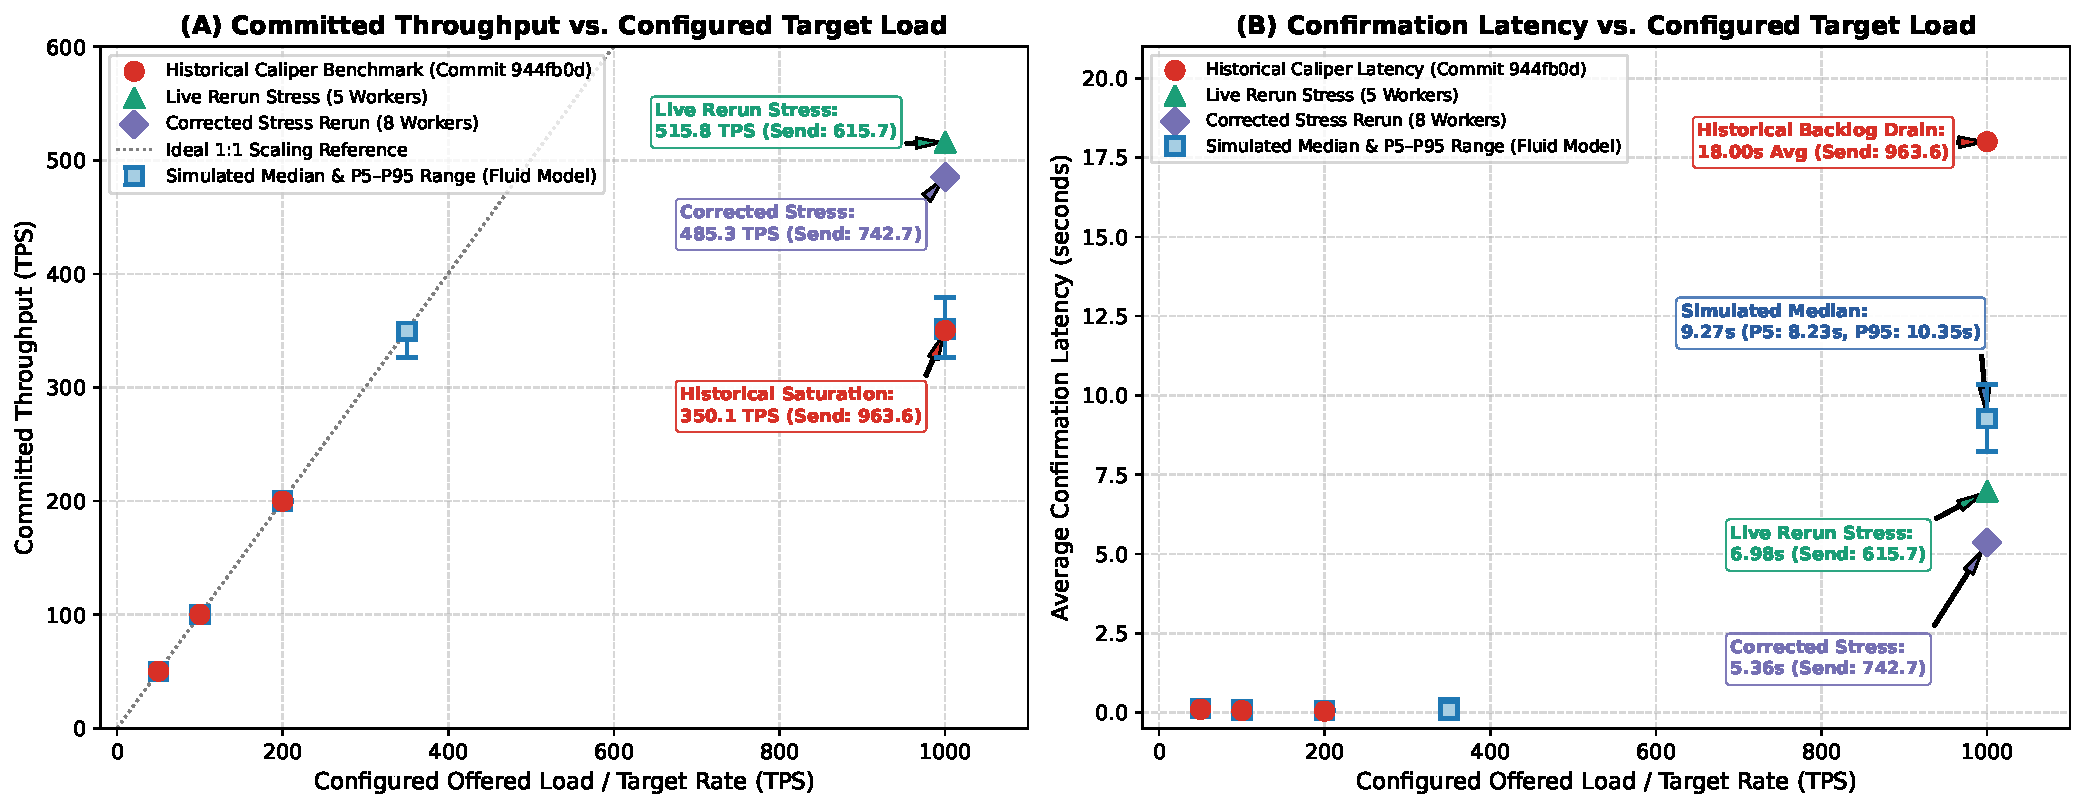
\includegraphics[width=\textwidth]{fig5b_caliper_simulation_projection.pdf}
\caption{Synthetic fluid-queueing simulation projections vs.\ empirical Caliper benchmarks plotted across configured target load (50, 100, 200, 350, and 1,000 TPS). Blue squares depict median simulated performance across 100 pseudo-random seeds, with vertical interval bars showing the exact P5--P95 simulation sensitivity range derived from the recorded fluid-queueing model outputs (\url{caliper-benchmark/results/simulated/20261018-011500/simulation_results.json}). These percentiles describe synthetic model sensitivity and are not empirical confidence intervals from repeated physical-network measurements. Distinct empirical benchmark runs are plotted at their configured target load with observed send rates annotated for the 1,000 TPS stress condition: historical single-client baseline (963.6 TPS send), 5-worker isolated testbed rerun (615.7 TPS send), and corrected 8-worker stress repetitions (742.7 TPS send).}\label{fig:sim_projection}
\end{figure}

\begin{figure}[t]
\centering
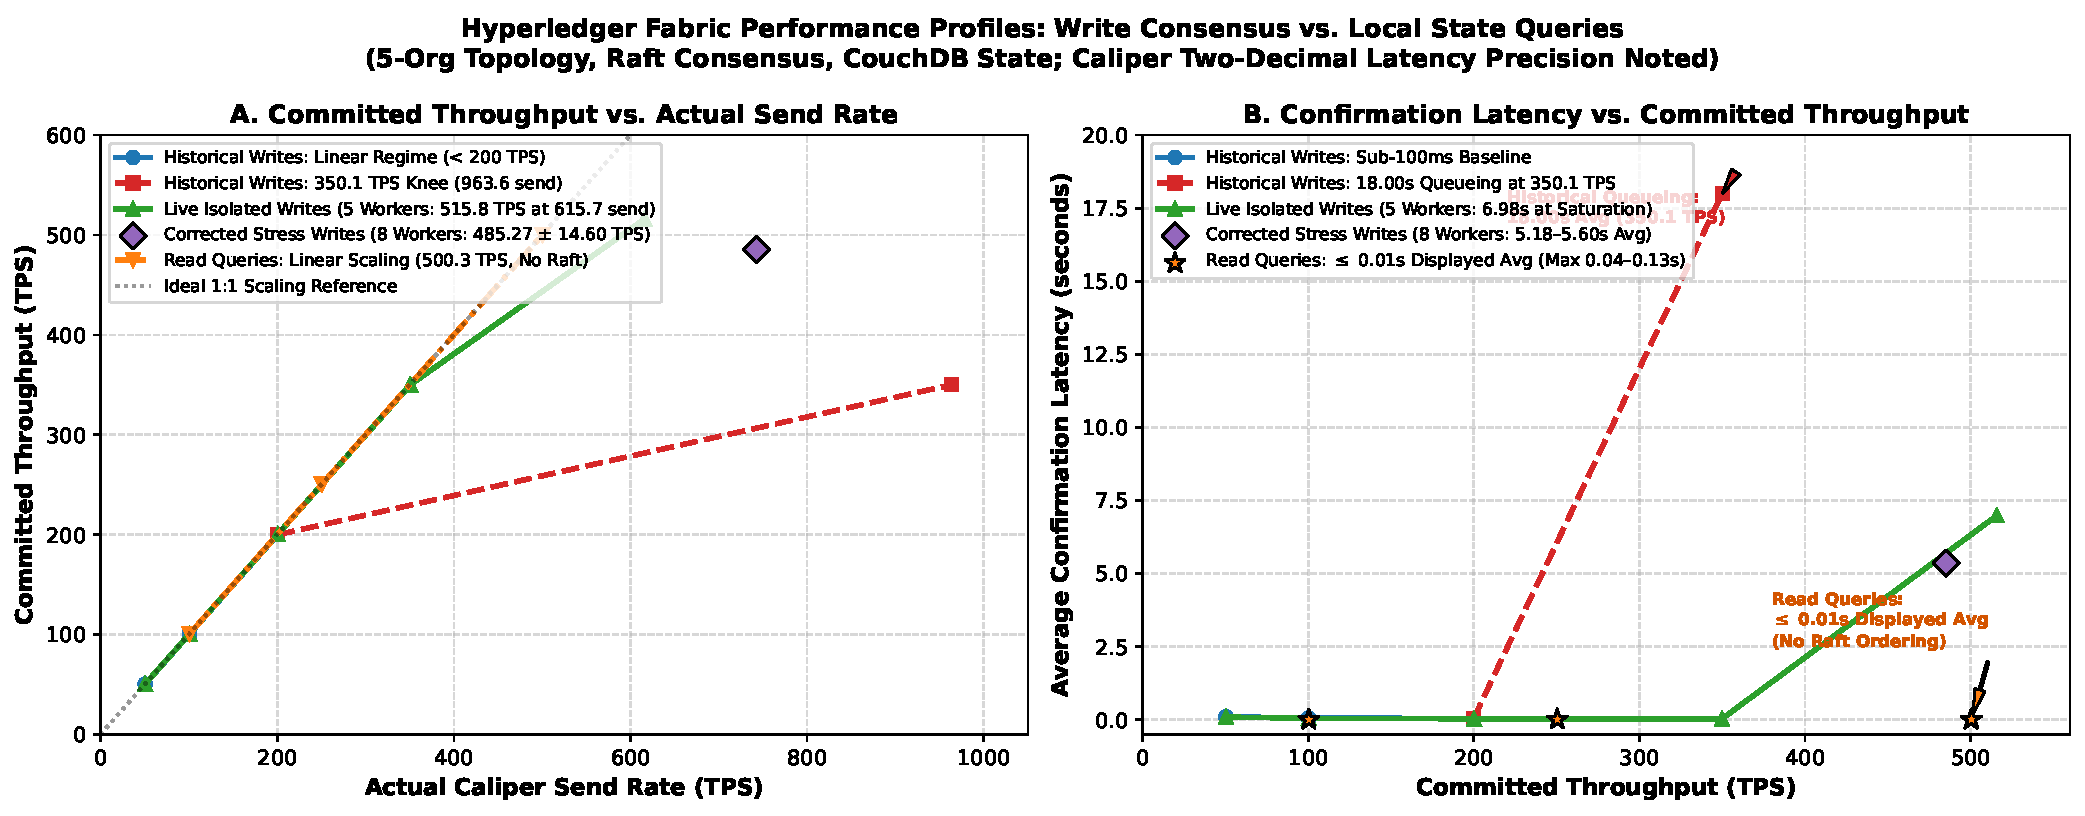
\includegraphics[width=\textwidth]{fig5_blockchain_benchmarks.pdf}
\caption{Hyperledger Fabric empirical performance profiles: Committed throughput and confirmation latency vs.\ actual send rate for write consensus vs.\ local state queries.}\label{fig:blockchain_benchmarks}
\end{figure}

\subsection{Analysis of Performance Regimes and End-to-End Application Throughput Boundary (RQ1 \& RQ2)}
Both empirical runs (visualized in Fig.~\ref{fig:blockchain_benchmarks}) and the queueing model reveal four key operational findings:
\begin{enumerate}
    \item \textbf{Linear Throughput Regime ($0 \to 200$ TPS):} For all write transactions submitted up to $200$ TPS, committed throughput tracks the offered rate linearly ($199.9$--$200.2$ TPS) with confirmation latency bounded between $0.03$s and $0.10$s (\texttt{MaxMessageCount = 10}, \texttt{BatchTimeout = 2.0s}).
    \item \textbf{Cross-Function Write Invariance:} At $200$ TPS, write throughput is virtually identical across \texttt{createPatientRecord} ($199.9$--$200.2$ TPS), \texttt{updateHealthScore} ($200.0$--$200.1$ TPS), \texttt{createPrescription} ($200.0$--$200.2$ TPS), and \texttt{requestScan} ($200.0$--$200.2$ TPS), confirming that confirmation time is governed by Raft ordering and peer validation rather than chaincode logic.
    \item \textbf{Empirical Saturation Dynamics and Decoupled Read Scalability:} Under nominal 1,000 TPS target load, write throughput saturates at $350.1$ TPS ($18.00$s latency) in the historical baseline, $515.8$ TPS ($6.98$s latency) in the 5-worker rerun, and $485.27 \pm 14.60$ TPS ($5.36 \pm 0.22$s latency) in the 8-worker repetitions with $0.00\%$ transaction failure rate among submitted proposals. Read queries (\texttt{getPatientRecord}) bypass ordering and reach $500.3$--$500.6$ TPS ($\le 0.01$s displayed average latency).
    \item \textbf{Chaincode Throughput vs.\ End-to-End Application Throughput:} While Fabric chaincode sustains $350$--$515$ write TPS at the Gateway SDK level, the off-chain Python ML inference engine requires $\approx 40$--$50$ ms per request to load models, engineer features, predict expenditure, and simulate loss. Analytically, a single synchronously awaiting Node.js worker process is bounded to:
    \begin{equation}
    \text{Capacity}_{\text{single-worker}} \approx \frac{1.0}{0.045\text{s}} \approx 20\text{--}25\text{ requests per second}
    \end{equation}
    Production deployments must therefore decouple ML inference from ledger writing via asynchronous message queues.
\end{enumerate}

% -----------------------------------------------------------------------------
\section{ACG-Inspired Chronic-Condition Feature Engineering, ML Evaluation, and Probability Threshold Sensitivity Analysis}
% -----------------------------------------------------------------------------

\subsection{Data Cohorts, Splitting Pipeline, and Forensic Overlap Audit}
We evaluate our machine learning pipeline across $46,458$ total records drawn from three official Agency for Healthcare Research and Quality (AHRQ) Medical Expenditure Panel Survey (MEPS) public-use files~\cite{ahrq_meps_2023}:
\begin{enumerate}
    \item \textbf{Development \& Held-Out Test Cohort (\texttt{MEPS HC-251}, 2023 Full-Year Consolidated):} Contains $18,919$ raw records; removing $148$ ineligible rows with \texttt{AGE23X < 0} yields \textbf{$N = 18,771$ eligible individuals} (retaining all $2,598$ zero-expenditure records [$13.84\%$] to prevent selection bias). Using an 80/20 random partition (\texttt{train\_test\_split}, \texttt{random\_state=42}), \texttt{HC-251} is divided into a \textbf{Training Split ($N = 15,016$)} and a \textbf{Held-Out Test Split ($N = 3,755$)}.
    \item \textbf{Cross-Year \& Unseen Panel External Cohort (\texttt{MEPS HC-256}, 2024 Full-Year Consolidated):} Contains \textbf{$N = 18,979$ eligible individuals}. Because MEPS uses an overlapping two-year rotating panel design, our forensic audit of person (\texttt{DUPERSID}) and household dwelling unit (\texttt{DUID}) identifiers established that \texttt{HC-256} comprises \textbf{Panel 28} ($N = 8,942$, Year 2, of whom $8,775$ [$46.24\%$ of \texttt{HC-256}] also appeared in \texttt{HC-251}: $7,030$ in Train and $1,745$ in Test) and \textbf{Panel 29} ($N = 10,037$, newly enrolled in 2024). Isolating \textbf{\texttt{HC-256} Panel 29 ($N = 10,037$)} provides a \textbf{$100\%$ disjoint external validation cohort with zero person (\texttt{DUPERSID}) and zero household (\texttt{DUID}) overlap} with \texttt{HC-251}.
    \item \textbf{Prospective Longitudinal Cohort (\texttt{MEPS HC-257}, Panel 28 Two-Year Longitudinal File, 2023--2024):} Tracks \textbf{$N = 8,708$ Panel 28 respondents} longitudinally to evaluate Year-2 expenditure forecasting (\texttt{TOTEXPY2}) from Year-1 baseline predictors. All $8,708$ respondents overlap with \texttt{HC-251} ($6,981$ in Train, $1,727$ in Test), establishing prospective within-subject temporal stability rather than unseen population transfer.
\end{enumerate}

\noindent\textit{Household (\texttt{DUID}) Split Disclosure:} Within \texttt{HC-251} ($N=18,771$ across $8,851$ unique households \texttt{DUID}), person-level \texttt{DUPERSID} overlap between Train ($N=15,016$) and Test ($N=3,755$) is strictly $0$. However, because \texttt{split\_data()} performs row-level splitting without grouping by \texttt{DUID}, $2,198$ households span Train and Test ($2,711 / 3,755$ test respondents [$72.20\%$] share a household \texttt{DUID} with at least one training respondent). To verify that shared household membership does not inflate model performance or distort threshold selection, we evaluate both \textbf{5-Fold Stratified Out-of-Fold (OOF) cross-validation} and \textbf{5-Fold Household-Grouped (\texttt{GroupKFold} by \texttt{DUID}) OOF cross-validation} strictly within the training split ($N=15,016$).

\subsection{Feature Definitions and Input Availability Parity}
HealthScore maps patient clinical indicators into 11 observable features adhering strictly to \textbf{Input Availability Parity} (excluding unobservable Self-Administered Questionnaire [SAQ] variables \texttt{Frailty\_Index}, \texttt{Age\_x\_Frailty}, and \texttt{K6SUM42} from the serving pipeline):
\begin{align}
\text{Cardio\_ACG} &= \text{HIBPDX} + \text{CHDDX} + \text{MIDX} + \text{STRKDX} \; (0\text{--}4) \\
\text{Metabolic\_ACG} &= \text{DIABDX\_M18} + \text{CHOLDX} \; (0\text{--}2) \\
\text{Respiratory\_ACG} &= \text{ASTHDX} + \text{EMPHDX} + \text{CHBRON31} \; (0\text{--}3) \\
\text{Oncology\_ACG} &= \text{CANCERDX} \; (0\text{--}1) \\
\text{Musculoskeletal\_ACG} &= \text{ARTHDX} + \text{JTPAIN31\_M18} \; (0\text{--}2) \\
\text{Psychiatric\_ACG} &= (\text{ADDPRS42} \in [1,2,3]) + \text{ADHDADDX} \; (0\text{--}2) \\
\text{Comorbidity\_Count} &= \sum_{c=1}^6 \mathbb{I}(\text{Cluster}_c > 0) \; (0\text{--}6) \\
\text{Multimorbidity\_Penalty} &= (\text{Comorbidity\_Count})^2 \; (0\text{--}36) \\
\text{Age\_x\_Comorbidity} &= \min(\text{Age}, 85) \times \text{Comorbidity\_Count} \; (0\text{--}510)
\end{align}
combined with continuous age (\texttt{AGE23X}, top-coded at 85) and binary sex (\texttt{Gender\_Male}). Absence of condition mentions in runtime intake is encoded as an uninformative zero default representing unobserved baseline status rather than confirmed clinical wellness, and these clusters are heuristic survey aggregations inspired by ACG concepts rather than an official Johns Hopkins ACG grouper.

\subsection{Controlled Feature Ablation Study and Model Selection (RQ3)}
To evaluate the isolated incremental contribution of each architectural component, we executed 17 controlled ablation experiments on the held-out MEPS HC-251 test partition ($N=3,755$). All models were refit on training data under identical hyperparameters (Tweedie GLM with power $p=1.5, \alpha=1.0$; Logistic Regression on Target 2 survey-weighted P90 with normalized sampling weights), as reported in Table~\ref{tab:ablations} and visualized in Fig.~\ref{fig:feature_ablations} and Fig.~\ref{fig:shap_importance}. Moving from demographics alone to the 6 chronic-condition clusters provides the primary predictive improvement: dollar $R^2$ increases from $0.0395$ to $0.0771$ ($\Delta R^2 = +0.0376$), and weighted BSS increases from $+0.0506$ to $+0.1005$ ($\Delta \text{BSS} = +0.0499$), whereas composite interaction terms yield modest incremental variance explanation ($\Delta R^2 = +0.0027$) despite dominating tree-based SHAP attribution ($39.0\%$).

\begin{table}[t]
\centering
\caption{Controlled feature ablation experiments on the held-out MEPS HC-251 test partition ($N=3,755$).}\label{tab:ablations}
\resizebox{\textwidth}{!}{%
\begin{tabular}{lclcccc}
\toprule
\textbf{Ablation Model Specification} & \textbf{Feats} & \textbf{Features Included} & \textbf{Dollar $R^2$} & $\Delta R^2$ & \textbf{Wtd BSS} & \textbf{ROC-AUC} \\
\midrule
\textbf{Full Observable Reference} & \textbf{11} & All 11 Observable Features & \textbf{0.0798} & \textbf{0.0000} & \textbf{+0.1025} & \textbf{0.7654} \\
Demographics Only & 2 & \texttt{AGE23X}, \texttt{Gender\_Male} & 0.0395 & -0.0403 & +0.0506 & 0.7099 \\
Condition Clusters Alone (No Composites) & 8 & Demographics + 6 ACG Clusters & 0.0771 & -0.0027 & +0.1005 & 0.7640 \\
Clusters + Comorbidity Count & 9 & Demographics + 6 Clusters + Count & 0.0787 & -0.0011 & +0.1004 & 0.7641 \\
Clusters + Multimorbidity Penalty & 9 & Demographics + 6 Clusters + $\text{Count}^2$ & 0.0769 & -0.0029 & +0.1017 & 0.7648 \\
Clusters + Age $\times$ Comorbidity & 9 & Demographics + 6 Clusters + Age $\times$ Count & 0.0766 & -0.0032 & +0.1007 & 0.7643 \\
Without Multimorbidity Penalty & 10 & 11 Features minus $\text{Count}^2$ & 0.0783 & -0.0015 & +0.1009 & 0.7649 \\
Without Age $\times$ Comorbidity & 10 & 11 Features minus Age $\times$ Count & \textbf{0.0804} & \textbf{+0.0006} & \textbf{+0.1027} & \textbf{0.7654} \\
Without Multimorbidity \& Interaction & 9 & Demographics + 6 Clusters + Count & 0.0787 & -0.0011 & +0.1004 & 0.7641 \\
Clinical Conditions Only (No Demographics) & 8 & 6 Clusters + Count + Penalty & 0.0791 & -0.0007 & +0.0996 & 0.7619 \\
Without Cardiovascular & 10 & 11 Features minus \texttt{Cardio\_ACG} & 0.0785 & -0.0013 & +0.0970 & 0.7634 \\
Without Metabolic & 10 & 11 Features minus \texttt{Metabolic\_ACG} & 0.0792 & -0.0006 & +0.0957 & 0.7628 \\
Without Respiratory & 10 & 11 Features minus \texttt{Respiratory\_ACG} & 0.0764 & -0.0035 & +0.0979 & 0.7635 \\
Without Oncology & 10 & 11 Features minus \texttt{Oncology\_ACG} & 0.0788 & -0.0010 & +0.0969 & 0.7645 \\
Without Musculoskeletal & 10 & 11 Features minus \texttt{Musculoskeletal\_ACG} & 0.0802 & +0.0004 & +0.1012 & 0.7651 \\
Without Psychiatric Condition & 10 & 11 Features minus \texttt{Psychiatric\_ACG} & 0.0774 & -0.0024 & +0.1026 & 0.7653 \\
\textbf{Oracle 14 Features (Upper Bound)} & \textbf{14} & Observable + SAQ Survey Variables & \textbf{0.0927} & \textbf{+0.0129} & \textbf{+0.1314} & \textbf{0.7904} \\
\bottomrule
\end{tabular}%
}
\end{table}

\begin{figure}[t]
\centering
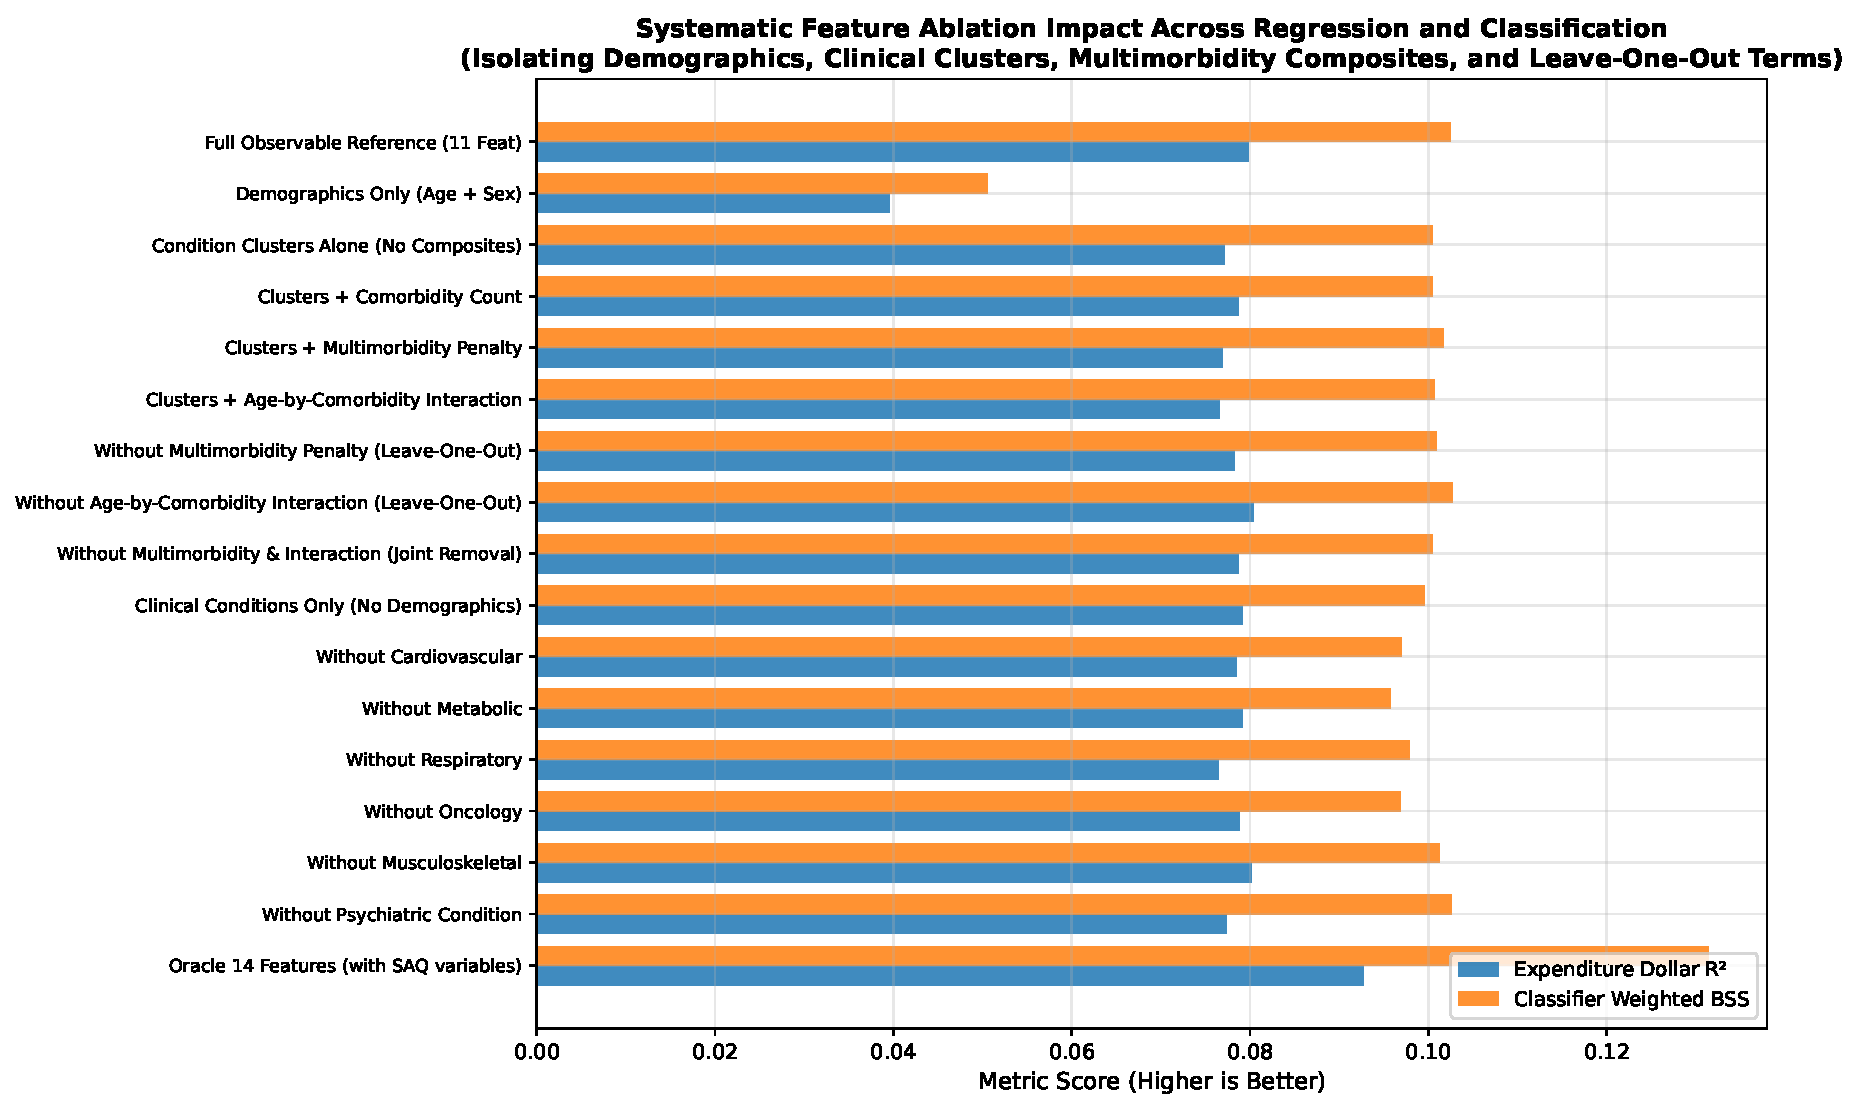
\includegraphics[width=\textwidth]{fig4_feature_ablations.pdf}
\caption{Systematic feature ablation comparison across expenditure dollar $R^2$ and high-cost classification weighted Brier Skill Score.}\label{fig:feature_ablations}
\end{figure}

\begin{figure}[t]
\centering
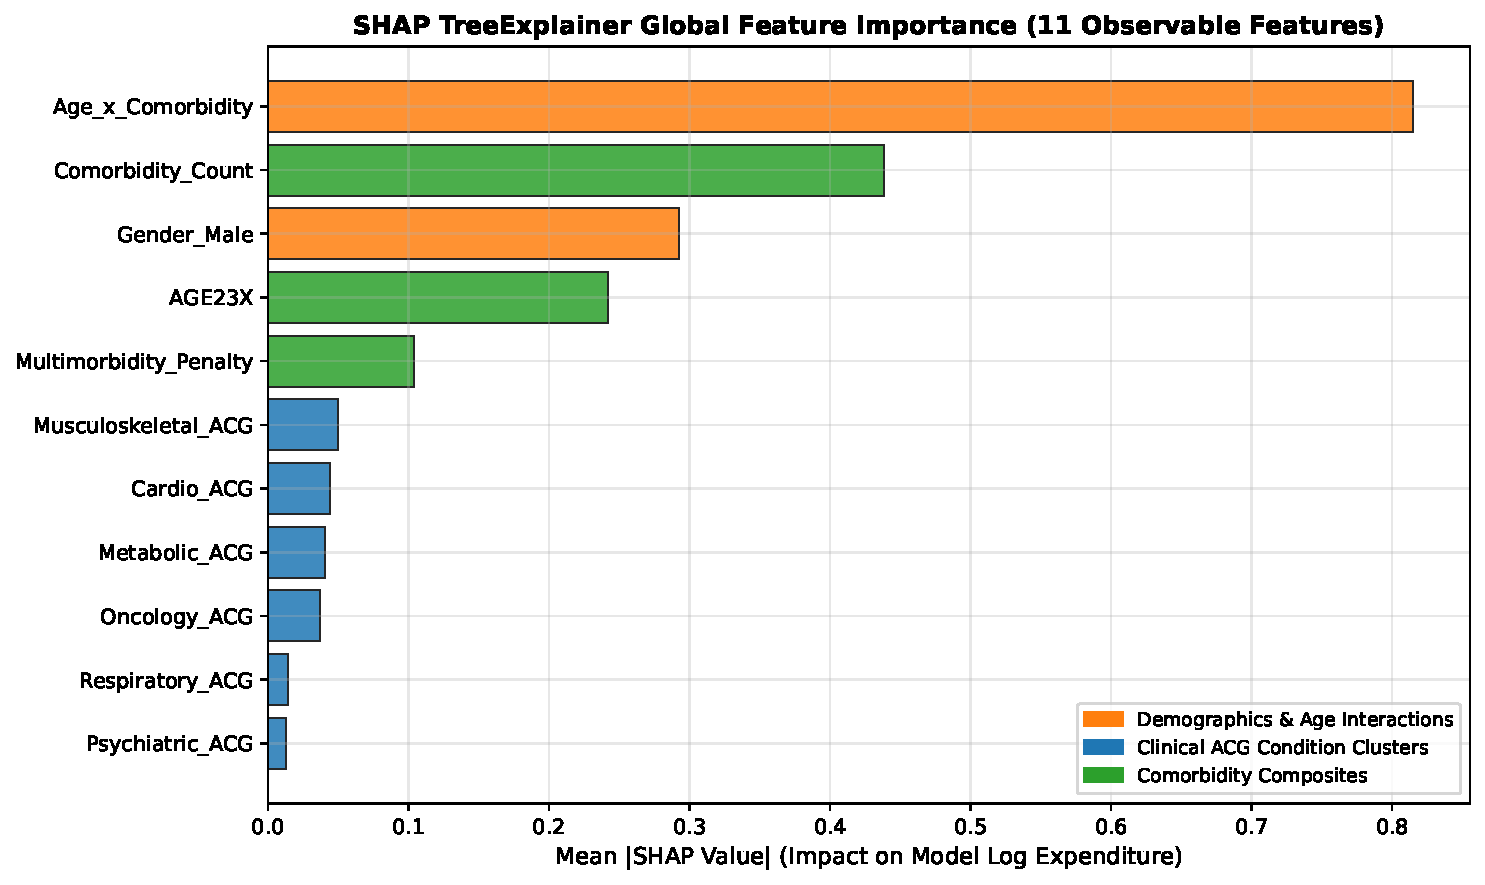
\includegraphics[width=0.88\textwidth]{fig3_shap_importance.pdf}
\caption{SHAP TreeExplainer global feature importance rankings across 11 observable features~\cite{lundberg2017unified}.}\label{fig:shap_importance}
\end{figure}

\paragraph{Target Definition Rationale and Classifier Comparison.}
In MEPS, the top decile of spenders accounts for approximately 65--70\% of total national medical expenditures. We define the primary high-expenditure target (\textbf{Target 2}) at the locked training survey-weighted 90th percentile ($\text{TOTEXP23} \ge \$17,827.41$; unweighted training P90 Target 1 is $\$20,360.50$). On the training split ($N=15,016$), survey-weighted positive prevalence is $9.99\%$ ($0.0999$) and unweighted prevalence is $11.56\%$ ($1,736 / 15,016$). On the held-out test partition ($N=3,755$), survey-weighted prevalence is $10.51\%$ ($0.1051$) and unweighted prevalence is $11.98\%$ ($450 / 3,755$), with constant-prediction baseline Brier scores~\cite{brier1950verification} of $0.0941$ (weighted) and $0.1059$ (unweighted). Table~\ref{tab:classifier_comparison} summarizes the 9 candidate classification models, and Fig.~\ref{fig:roc_pr_curves} and Fig.~\ref{fig:calibration_deciles} illustrate discrimination and calibration~\cite{steyerberg2010assessing}.

\begin{table}[t]
\centering
\caption{Candidate classification model comparison on the fixed held-out MEPS HC-251 test partition ($N=3,755$, Target 2: Survey-Weighted P90 $\ge \$17,827.41$).}\label{tab:classifier_comparison}
\resizebox{\textwidth}{!}{%
\begin{tabular}{lclccccccccc}
\toprule
\textbf{Candidate Classifier} & \textbf{Feats} & \textbf{Weighting Policy} & \textbf{ROC-AUC [95\% CI]} & \textbf{PR-AUC [95\% CI]} & \textbf{Unw Brier} & \textbf{Wtd Brier} & \textbf{Wtd BSS} & \textbf{CITL ($\alpha$)} & \textbf{Cal Slope ($\beta$)} & \textbf{Prec@0.10} & \textbf{Rec@0.10} \\
\midrule
Constant Prevalence Baseline                     & 0  & Constant $\hat{p}=0.0999$          & 0.5000 [0.5000, 0.5000] & 0.1198 [0.1111, 0.1308] & 0.1059 & 0.0941 & +0.0000 & 0.0000  & 0.0000 & 0.0000 & 0.0000 \\
Demographic Baseline                            & 2  & \texttt{AGE23X}, \texttt{Gender}   & 0.7099 [0.6856, 0.7319] & 0.2182 [0.1928, 0.2489] & 0.0996 & 0.0893 & +0.0506 & +0.0388 & 0.8859 & 0.1949 & 0.7867 \\
Clinical Conditions Only                        & 8  & 6 Clusters + Count + Penalty       & 0.7619 [0.7393, 0.7847] & 0.3083 [0.2794, 0.3464] & 0.0941 & 0.0847 & +0.0996 & +0.0768 & 0.9539 & 0.2291 & 0.7622 \\
\textbf{Logistic (11-Feat Observable, Wtd Fit)} & \textbf{11} & \textbf{Frozen Normalized Weights (Serving)} & \textbf{0.7654} [0.7444, 0.7881] & \textbf{0.3184} [0.2876, 0.3556] & \textbf{0.0936} & \textbf{0.0845} & \textbf{+0.1025} & \textbf{+0.0646} & \textbf{0.9438} & \textbf{0.2318} & \textbf{0.7733} \\
\textit{Logistic (11-Feat Observable, Unw Fit)} & 11 & Unweighted Fit (Weighting Ablation) & 0.7652 [0.7433, 0.7882] & 0.3192 [0.2869, 0.3582] & 0.0936 & 0.0845 & +0.1025 & +0.0570 & 0.9008 & 0.2278 & 0.7644 \\
Random Forest (11-Feat Observable)              & 11 & Normalized Person Weights          & 0.7693 [0.7458, 0.7928] & 0.3157 [0.2823, 0.3550] & 0.0935 & 0.0841 & +0.1062 & +0.0601 & 0.9736 & 0.2342 & 0.7556 \\
XGBoost (Uncalibrated)                          & 11 & Normalized Person Weights          & 0.7705 [0.7482, 0.7940] & 0.3196 [0.2853, 0.3598] & 0.0932 & 0.0838 & +0.1093 & +0.0572 & 0.9926 & 0.2262 & 0.8022 \\
Platt-Calibrated XGBoost                        & 11 & Observable, Sigmoid CV=5           & 0.7702 [0.7472, 0.7936] & 0.3183 [0.2872, 0.3580] & 0.0944 & 0.0847 & +0.0998 & +0.0617 & 1.0335 & 0.2535 & 0.6778 \\
Logistic (14-Feat Oracle)                       & 14 & Observable + SAQ Survey            & 0.7904 [0.7684, 0.8121] & 0.3472 [0.3143, 0.3917] & 0.0922 & 0.0832 & +0.1159 & +0.0493 & 1.0609 & 0.2806 & 0.6822 \\
\bottomrule
\end{tabular}%
}
\vspace{1mm}
\raggedright\scriptsize{Note: 95\% confidence intervals derive from non-parametric row-level bootstrap resampling ($B=200$, seed 42) matching \texttt{experiment\_registry.json}. The approved serving candidate is the frozen weighted model (\texttt{risk\_model\_classifier\_observable\_weighted\_p90.pkl}). Calibration-in-the-large (CITL, $\alpha$) is estimated via exact Brent root-solving with slope fixed at 1 ($\sum w_i (y_i - \sigma(\alpha + \text{logit}(p_i))) = 0$). For the weighted candidate, bivariate logistic calibration yields intercept $a = -0.0409$ and slope $b = 0.9438$.}
\end{table}

\begin{figure}[t]
\centering
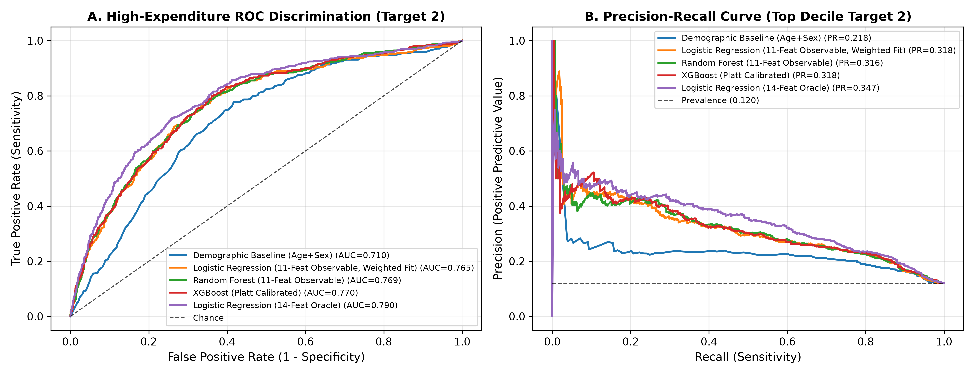
\includegraphics[width=\textwidth]{fig1_roc_pr_curves.pdf}
\caption{Receiver Operating Characteristic (ROC) and Precision--Recall (PR) curves for high-expenditure classification across candidate models.}\label{fig:roc_pr_curves}
\end{figure}

\begin{figure}[t]
\centering
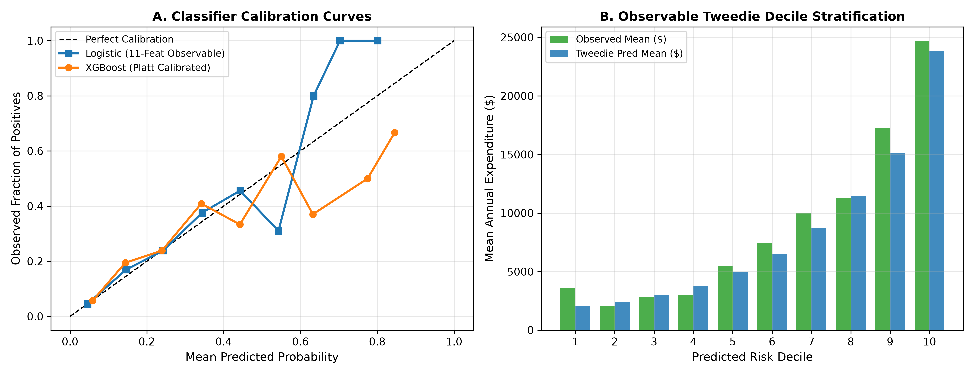
\includegraphics[width=\textwidth]{fig2_calibration_deciles.pdf}
\caption{(A) Classifier calibration curves and (B) Observable Tweedie decile expenditure stratification comparing observed and predicted expenditures.}\label{fig:calibration_deciles}
\end{figure}

The 11-feature Observable Logistic Regression (Weighted Fit) was selected as the deployment candidate based on input availability parity, superior skill over conditional-expectation imputation ($+0.1025$ vs $+0.0978$), calibration quality ($b = 0.9438$, $\text{CITL} = +0.0646$), and closed-form log-odds interpretability. While tree ensembles (Random Forest and XGBoost) achieve marginally higher point estimates on the test partition (ROC-AUC $0.7693$--$0.7705$ vs $0.7654$) with overlapping marginal 95\% bootstrap confidence intervals, we make no claim of formal statistical significance or non-significance because paired hypothesis tests were not performed in the baseline registry.

\subsection{Classification Probability Threshold Sensitivity Analysis (RQ4)}
At the reference predicted-probability threshold of $\tau = 0.10$, the serving classifier (\texttt{risk\_model\_classifier\_observable\_weighted\_p90.pkl}, SHA-256: \texttt{3632f820...}) flags $1,501$ of $3,755$ test patients ($39.97\%$), capturing $348$ of $450$ true high-expenditure cases ($\text{Recall} = 77.33\%$) but generating $1,153$ false positives ($\text{Precision} = 23.18\%$, an unweighted enrichment of $1.93\times$ over the $11.98\%$ unweighted test prevalence; $\text{F1} = 0.3567$).

To investigate whether adjusting the classification cutoff provides a more useful precision--recall balance without altering the underlying fitted model, we evaluated the frozen serving model's predicted probabilities $\hat{p}_i$ across 12 probability thresholds: the required primary grid $\tau \in \{0.10, 0.20, 0.30, 0.40, 0.50, 0.60, 0.70, 0.80, 0.90\}$ plus three intermediate diagnostic cutoffs $\tau \in \{0.05, 0.15, 0.25\}$. Because \texttt{split\_data()} does not create a separate standalone validation split, selecting an operating threshold on the held-out test set ($N=3,755$) would constitute test-set leakage. We therefore executed \textbf{leak-free 5-fold Out-of-Fold (OOF) cross-validation strictly within the training split ($N=15,016$, $P=1,736$)} under both Stratified 5-Fold CV and Household-Grouped (\texttt{GroupKFold} by \texttt{DUID}) 5-Fold CV to select candidate operating thresholds prior to evaluating on the held-out test partition ($N=3,755$, $P=450$) and the strictly disjoint 2024 external cohort (\texttt{HC-256} Panel 29, $N=10,037$, $P=1,258$). Table~\ref{tab:threshold_sweep} reports the complete threshold comparison across OOF Validation, Held-Out Test, and Unseen External Panel 29, and Figs.~\ref{fig:t1}--\ref{fig:t4} visualize the resulting precision--recall curves, error counts, and confusion matrices.

\begin{table}[t]
\centering
\caption{Probability threshold sensitivity analysis of the frozen 11-feature Observable Logistic Regression classifier across 5-Fold Stratified Out-of-Fold Validation ($N=15,016$, $P=1,736$), Held-Out Test ($N=3,755$, $P=450$), and Strictly Unseen External 2024 Panel 29 ($N=10,037$, $P=1,258$).}\label{tab:threshold_sweep}
\resizebox{\textwidth}{!}{%
\begin{tabular}{cccccccccccccc}
\toprule
\textbf{Cutoff} & \textbf{5-Fold OOF Val ($N=15,016$)} & \multicolumn{4}{c}{\textbf{Held-Out Test Counts ($N=3,755$)}} & \textbf{Test Flagged} & \textbf{Test Unw Prec} & \textbf{Test Unw} & \textbf{Test Unw} & \textbf{Test Unw} & \textbf{Test Wtd} & \textbf{Unseen Panel 29 ($N=10,037$)} \\
\cmidrule(lr){3-6}
$\boldsymbol{\tau}$ & \textbf{Prec / Rec / F1 / BalAcc} & \textbf{TP} & \textbf{FP} & \textbf{TN} & \textbf{FN} & \textbf{$N$ (Unw / Wtd \%)} & \textbf{\% (Enrich / Ceil)} & \textbf{Rec / Spec \%} & \textbf{NPV \%} & \textbf{F1 / BalAcc} & \textbf{Prec / Rec / F1} & \textbf{Prec / Rec / F1 / Spec} \\
\midrule
0.05$^\dagger$ & 17.36\% / 89.92\% / 0.2910 / 0.6698 & 401 & 1,879 & 1,426 & 49  & 2,280 (60.72 / 55.01) & 17.59\% (1.47$\times$ / 19.74\%) & 89.11 / 43.15 & 96.68 & 0.2938 / 0.6613 & 15.98\% / 83.59\% / 0.2682 & 18.30\% / 91.02\% / 0.3047 / 41.77\% \\
\textbf{0.10}  & \textbf{22.78\% / 77.30\% / 0.3519 / 0.7152} & \textbf{348} & \textbf{1,153} & \textbf{2,152} & \textbf{102} & \textbf{1,501 (39.97 / 33.54)} & \textbf{23.18\% (1.93$\times$ / 29.98\%)} & \textbf{77.33 / 65.11} & \textbf{95.47} & \textbf{0.3567 / 0.7122} & \textbf{22.54\% / 71.93\% / 0.3433} & \textbf{23.78\% / 78.46\% / 0.3650 / 63.97\%} \\
0.15$^\dagger$ & 27.15\% / 63.08\% / 0.3796 / 0.7048 & 281 & 771   & 2,534 & 169 & 1,052 (28.02 / 21.89) & 26.71\% (2.23$\times$ / 42.78\%) & 62.44 / 76.67 & 93.75 & \textbf{0.3742} / 0.6956 & 26.09\% / 54.32\% / \textbf{0.3525} & 28.65\% / 66.14\% / 0.3998 / 76.40\% \\
\textbf{0.20}  & \textbf{31.28\% / 50.23\% / 0.3855 / 0.6790} & \textbf{211} & \textbf{481}   & \textbf{2,824} & \textbf{239} & \textbf{692 (18.43 / 13.76)}   & \textbf{30.49\% (2.54$\times$ / 65.03\%)} & \textbf{46.89 / 85.45} & \textbf{92.20} & \textbf{0.3695 / 0.6617} & \textbf{30.73\% / 40.23\% / 0.3485} & \textbf{32.69\% / 52.38\% / 0.4026 / 84.54\%} \\
0.25$^\dagger$ & 36.31\% / 38.59\% / 0.3742 / 0.6487 & 154 & 286   & 3,019 & 296 & 440 (11.72 / 8.77)    & 35.00\% (2.92$\times$ / 100.0\%) & 34.22 / 91.35 & 91.07 & 0.3461 / 0.6278 & 35.04\% / 29.25\% / 0.3188 & 37.77\% / 40.62\% / 0.3914 / 90.41\% \\
\textbf{0.30}  & \textbf{39.73\% / 26.73\% / 0.3196 / 0.6071} & \textbf{114} & \textbf{171}   & \textbf{3,134} & \textbf{336} & \textbf{285 (7.59 / 5.69)}     & \textbf{40.00\% (3.34$\times$ / 100.0\%)} & \textbf{25.33 / 94.83} & \textbf{90.32} & \textbf{0.3102 / 0.6008} & \textbf{40.10\% / 21.72\% / 0.2818} & \textbf{42.29\% / 30.29\% / 0.3529 / 94.08\%} \\
0.40           & 46.85\% / 11.98\% / 0.1908 / 0.5510 & 46  & 58    & 3,247 & 404 & 104 (2.77 / 2.02)     & 44.23\% (3.69$\times$ / 100.0\%) & 10.22 / 98.25 & 88.93 & 0.1661 / 0.5423 & 43.25\% / 8.33\% / 0.1397  & 47.53\% / 14.55\% / 0.2228 / 97.70\% \\
0.50           & 51.59\% / 4.67\% / 0.0856 / 0.5205  & 15  & 21    & 3,284 & 435 & 36 (0.96 / 0.71)      & 41.67\% (3.48$\times$ / 100.0\%) & 3.33 / 99.36  & 88.30 & 0.0617 / 0.5135 & 37.12\% / 2.52\% / 0.0472  & 53.33\% / 5.72\% / 0.1034 / 99.28\% \\
0.60           & 63.46\% / 1.90\% / 0.0369 / 0.5088  & 6   & 1     & 3,304 & 444 & 7 (0.19 / 0.11)       & 85.71\% (7.15$\times$ / 100.0\%) & 1.33 / 99.97  & 88.15 & 0.0263 / 0.5065 & 82.19\% / 0.84\% / 0.0166  & 63.41\% / 2.07\% / 0.0400 / 99.83\% \\
0.70           & 66.67\% / 0.35\% / 0.0069 / 0.5016  & 2   & 0     & 3,305 & 448 & 2 (0.05 / 0.04)       & 100.0\% (8.34$\times$ / 100.0\%) & 0.44 / 100.0  & 88.06 & 0.0088 / 0.5022 & 100.0\% / 0.39\% / 0.0078  & 100.0\% / 0.40\% / 0.0079 / 100.0\% \\
0.80           & 50.00\% / 0.06\% / 0.0012 / 0.5003  & 1   & 0     & 3,305 & 449 & 1 (0.03 / 0.03)       & 100.0\% (8.34$\times$ / 100.0\%) & 0.22 / 100.0  & 88.04 & 0.0044 / 0.5011 & 100.0\% / 0.24\% / 0.0048  & 100.0\% / 0.08\% / 0.0016 / 100.0\% \\
0.90           & 0.00\% / 0.00\% / 0.0000 / 0.5000   & 0   & 0     & 3,305 & 450 & 0 (0.00 / 0.00)       & 0.00\% (0.00$\times$ / ---)      & 0.00 / 100.0  & 88.02 & 0.0000 / 0.5000 & 0.00\% / 0.00\% / 0.0000   & 0.00\% / 0.00\% / 0.0000 / 100.0\% \\
\bottomrule
\end{tabular}%
}
\vspace{1mm}
\raggedright\scriptsize{$^\dagger$ Intermediate diagnostic thresholds ($\tau \in \{0.05, 0.15, 0.25\}$) evaluated alongside the required primary grid ($\tau \in \{0.10, 0.20, \dots, 0.90\}$). ``Ceil'' denotes the theoretical oracle maximum precision $\min(P, \text{Flagged}(\tau))/\text{Flagged}(\tau)$ achievable by a hypothetical perfect classifier ($\text{ROC-AUC}=1.0$) at that exact flagged volume. Bold rows indicate the three validated operational tiers ($\tau = 0.10$ max Balanced Accuracy screening, $\tau = 0.20$ primary-grid F1-optimal triage, and $\tau = 0.30$ high-specificity targeted intervention).}
\end{table}

\begin{figure}[t]
\centering
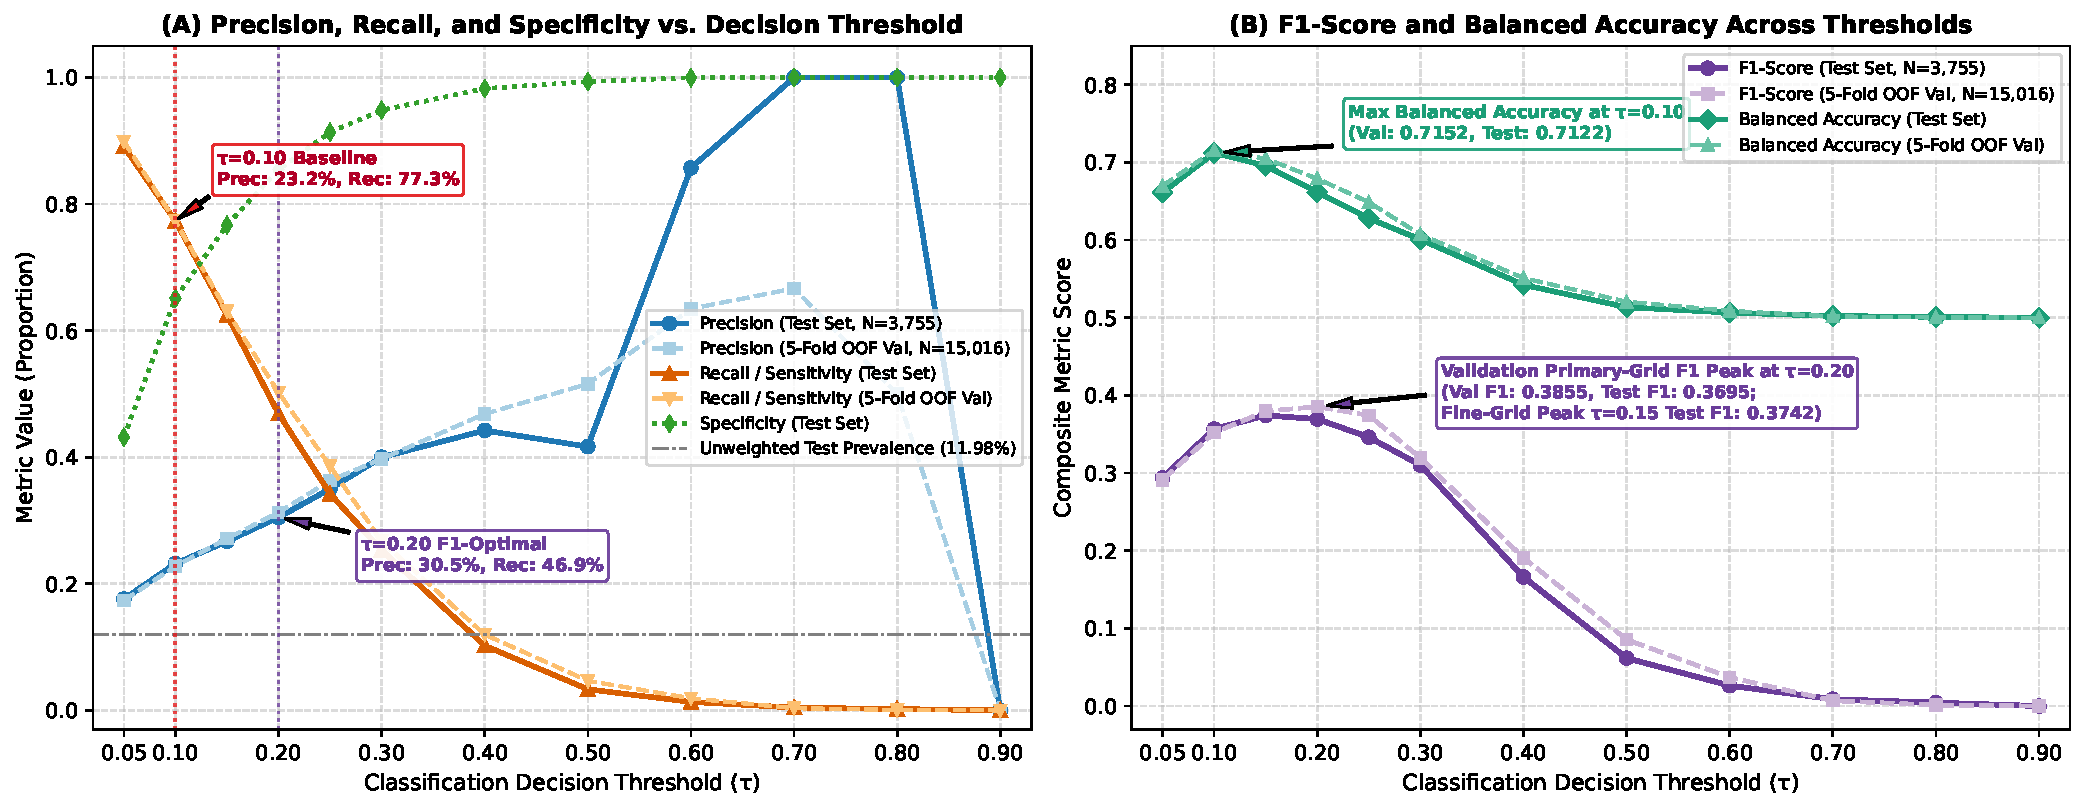
\includegraphics[width=\textwidth]{fig_t1_precision_recall_f1_vs_threshold.pdf}
\caption{(A) Precision, Recall, and Specificity and (B) F1-Score and Balanced Accuracy across decision thresholds $\tau \in [0.05, 0.90]$ on 5-Fold OOF Validation ($N=15,016$) and the Held-Out Test Set ($N=3,755$).}\label{fig:t1}
\end{figure}

\begin{figure}[t]
\centering
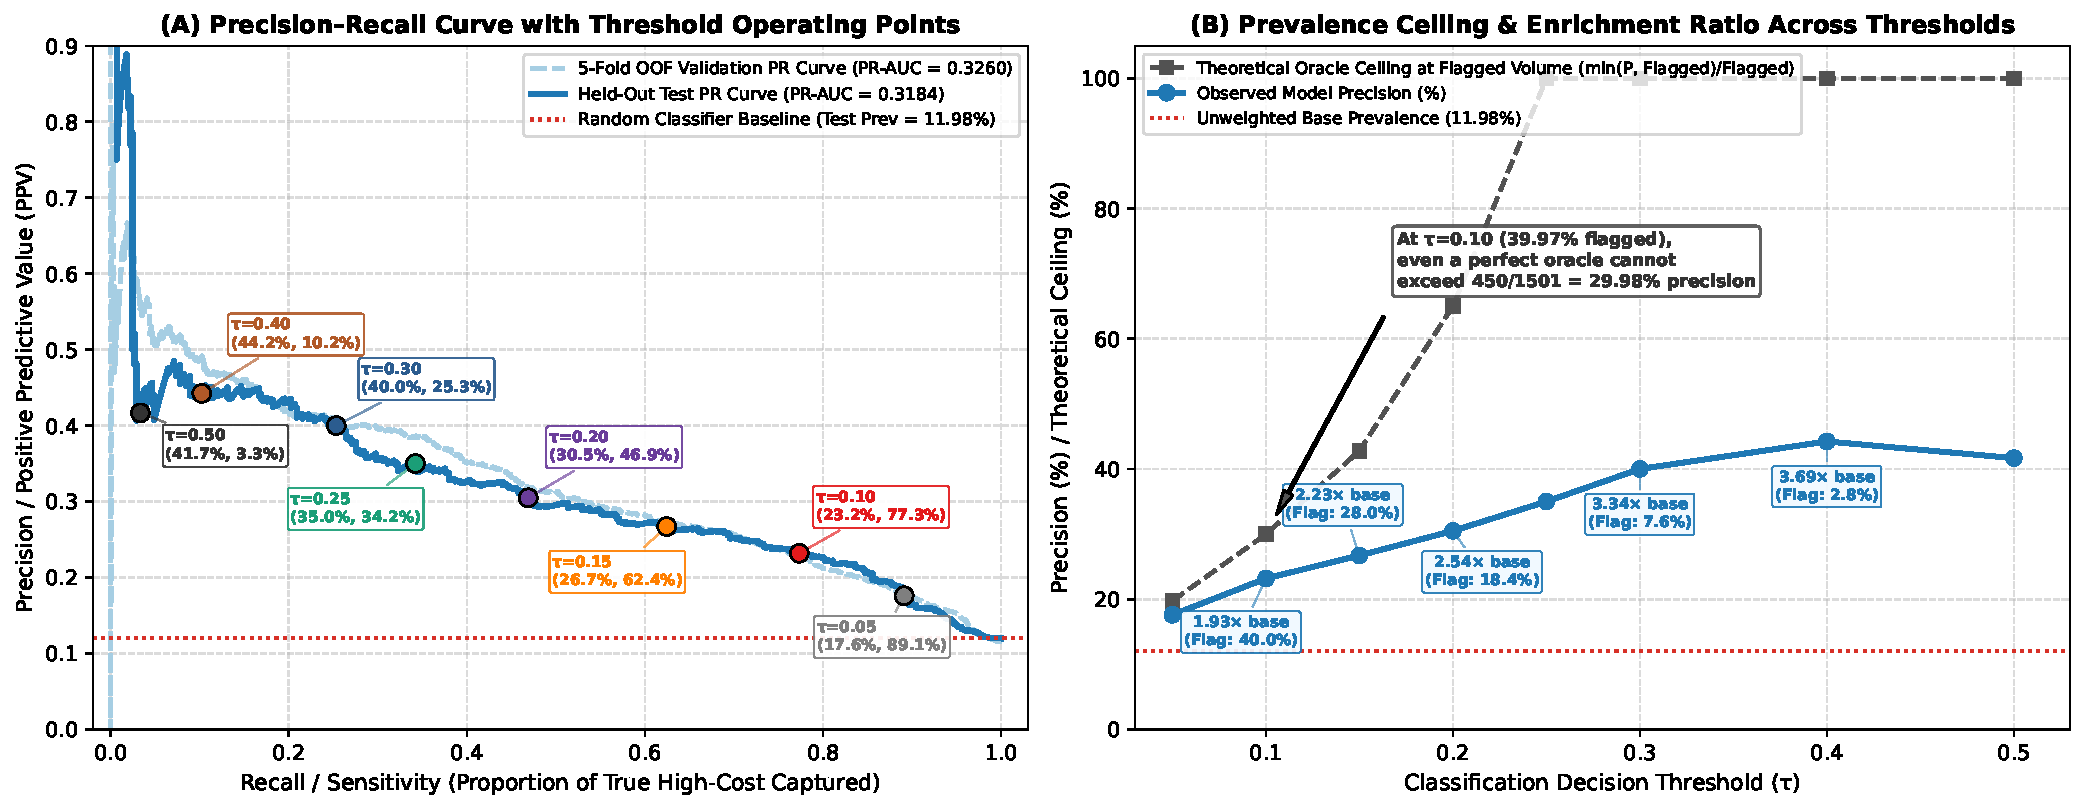
\includegraphics[width=\textwidth]{fig_t2_precision_recall_tradeoff.pdf}
\caption{(A) Precision--Recall curve overlaid with discrete threshold operating points ($\tau = 0.05$ to $0.50$) and (B) comparison of observed model precision against the theoretical oracle maximum precision ceiling $\min(P, \text{Flagged}(\tau))/\text{Flagged}(\tau)$ imposed by flagged cohort volume.}\label{fig:t2}
\end{figure}

\begin{figure}[t]
\centering
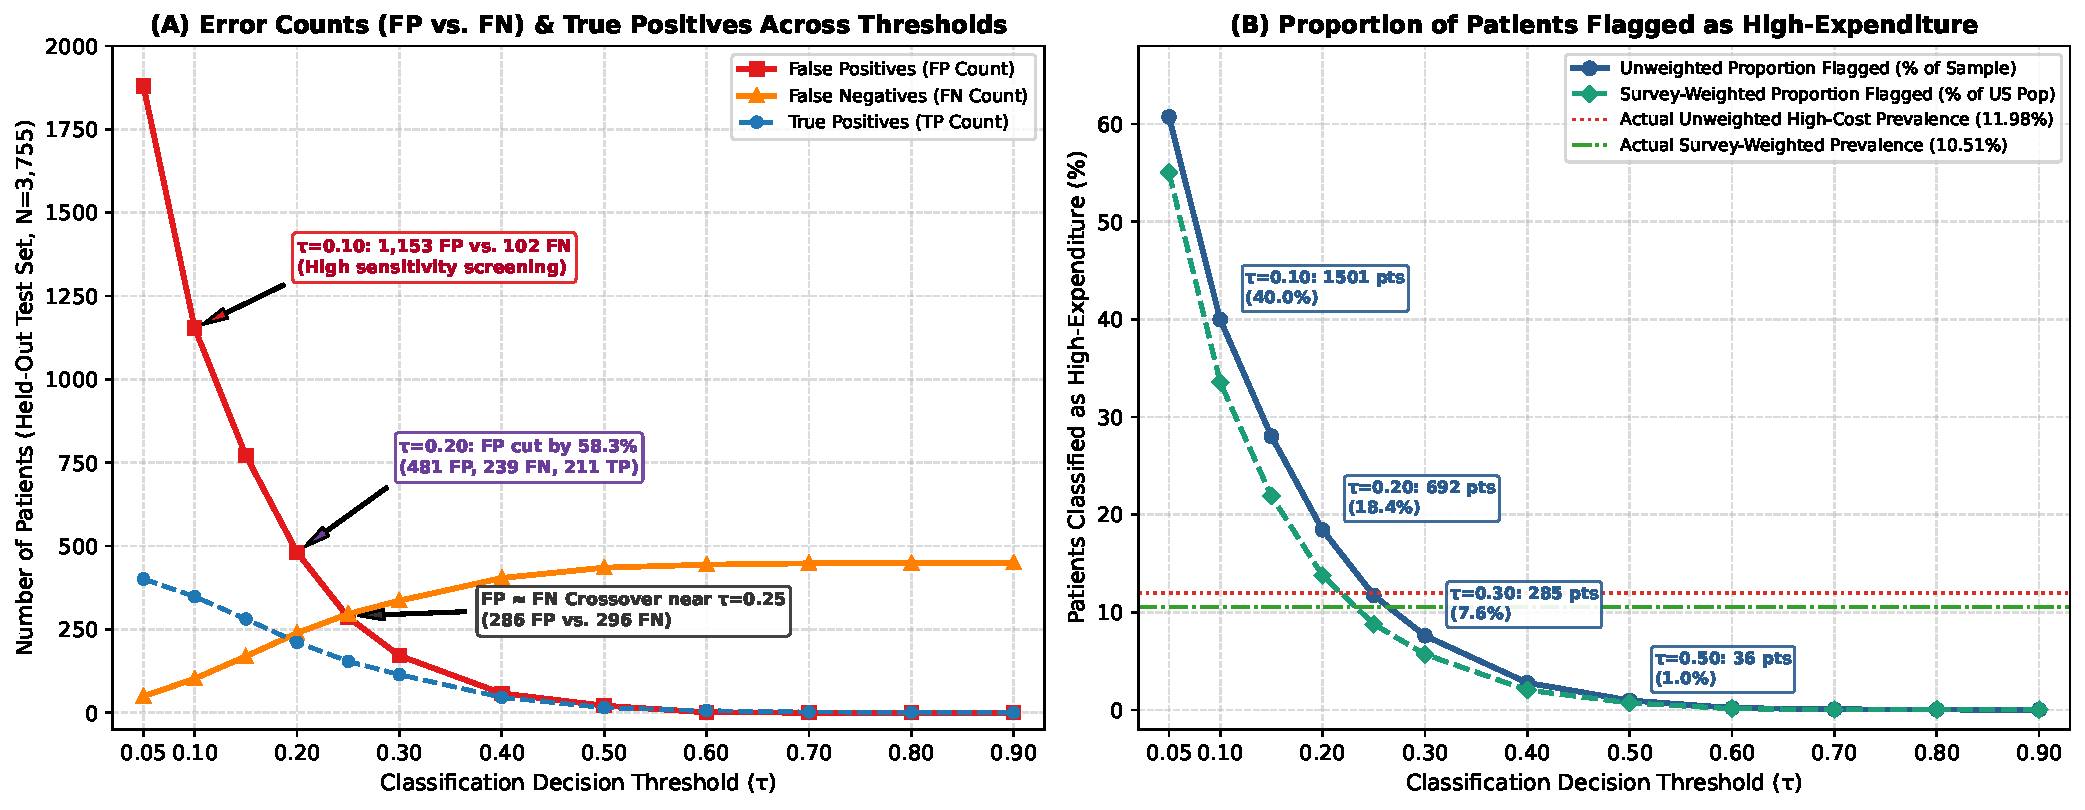
\includegraphics[width=\textwidth]{fig_t3_fp_fn_and_flagged_volume.pdf}
\caption{(A) Absolute False Positives ($\text{FP}$), False Negatives ($\text{FN}$), and True Positives ($\text{TP}$) and (B) unweighted vs.\ survey-weighted percentage of patients flagged as high-expenditure across thresholds $\tau \in [0.05, 0.90]$ on the held-out test set ($N=3,755$).}\label{fig:t3}
\end{figure}

\begin{figure}[t]
\centering
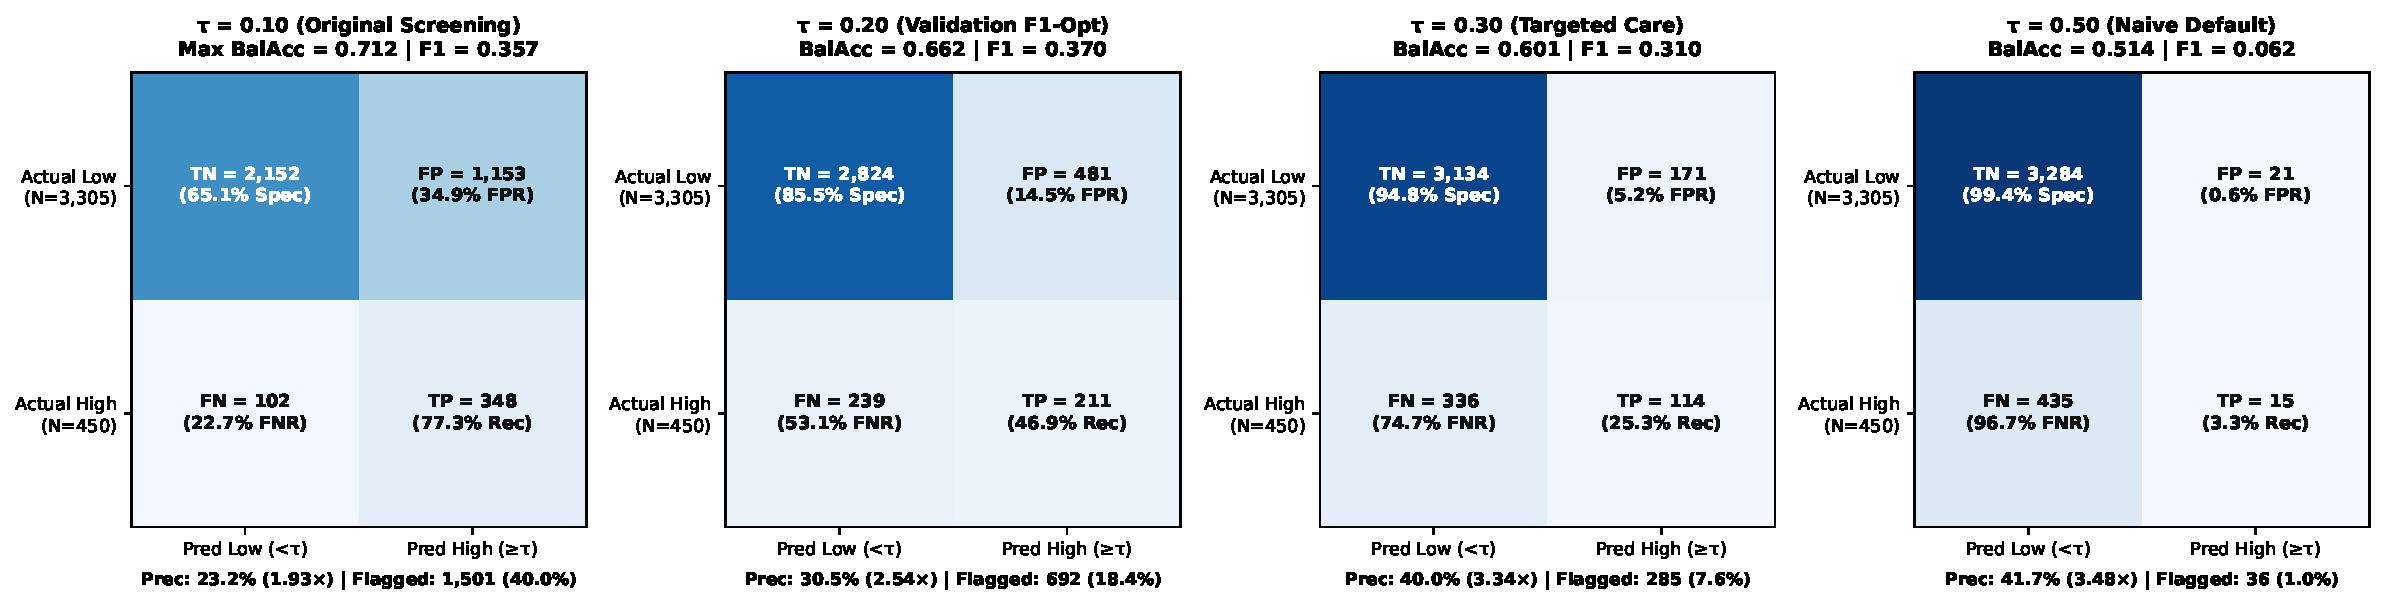
\includegraphics[width=\textwidth]{fig_t4_confusion_matrices_comparison.pdf}
\caption{Held-out test confusion matrices ($N=3,755$, $P=450$) at four representative operating points: $\tau = 0.10$ (Reference High-Sensitivity Screening, max Balanced Accuracy $= 0.7122$), $\tau = 0.20$ (Validation Primary-Grid F1-Optimal Triage, $\text{F1} = 0.3695$, $\text{FP}$ reduced by $58.28\%$), $\tau = 0.30$ (Targeted Intensive Case Management, $\text{Precision} = 40.00\%$, $\text{Specificity} = 94.83\%$), and $\tau = 0.50$ (Naive Default Cutoff, showing severe recall collapse to $3.33\%$).}\label{fig:t4}
\end{figure}

\subsection{Six-Factor Root-Cause Investigation of Precision at $\tau = 0.10$ and Operational Tiering}
Our diagnostic audit across all six required candidate factors establishes the exact mathematical and clinical mechanisms governing precision and recall across $\tau \in [0.05, 0.90]$:

\begin{enumerate}
    \item \textbf{Threshold Sensitivity and Mathematical Volume-Ceiling Bound (Primary Direct Cause):} Because $\tau = 0.10$ is set near the population base prevalence, $39.97\%$ of the test cohort ($1,501 / 3,755$ individuals; $33.54\%$ survey-weighted) have predicted probabilities $\hat{p}_i \ge 0.10$. However, the entire test partition contains only $P = 450$ true high-expenditure individuals ($11.98\%$). Consequently, \textbf{even a hypothetical perfect oracle classifier ($\text{ROC-AUC} = 1.00$, $100\%$ recall) that flags $1,501$ individuals cannot mathematically exceed a precision of:}
    \begin{equation}
    \text{Prec}_{\text{oracle}}(1{,}501) = \frac{\min(450, 1{,}501)}{1{,}501} = \frac{450}{1{,}501} = 29.98\%
    \end{equation}
    At $\tau = 0.10$, our serving classifier captures $348$ of the $450$ true positives ($\text{Recall} = 77.33\%$), achieving $348 / 1,501 = 23.18\%$ precision---which represents \textbf{$77.33\%$ of the theoretical maximum precision mathematically possible when screening $40\%$ of the cohort} (Fig.~\ref{fig:t2}B). When the threshold is raised to the OOF-selected primary-grid F1 optimum ($\tau = 0.20$, where OOF Validation F1 peaks at $0.3855$ unweighted and $0.3551$ weighted), the flagged test cohort contracts to $692$ patients ($18.43\%$ unweighted, $13.76\%$ weighted), \textbf{eliminating $672$ false positives (a $58.28\%$ reduction in $\text{FP}$, from $1,153$ to $481$)}, lifting test precision to \textbf{$30.49\%$ ($2.54\times$ enrichment; $32.69\%$ on unseen 2024 Panel 29)} and test F1 to \textbf{$0.3695$} while retaining $46.89\%$ recall ($50.23\%$ on OOF Validation, $52.38\%$ on unseen Panel 29). On the fine diagnostic grid, $\tau = 0.15$ achieves the highest held-out test F1 of \textbf{$0.3742$} ($26.71\%$ precision, $62.44\%$ recall, $33.13\%$ fewer false positives). Raising $\tau$ to $0.30$ further reduces false positives by \textbf{$85.17\%$} ($1,153 \to 171$, $\text{Specificity} = 94.83\%$) and elevates test precision to \textbf{$40.00\%$ ($3.34\times$ enrichment; $42.29\%$ on Panel 29)}.
    \item \textbf{Class Imbalance ($7.34:1$ Negative-to-Positive Conditioning):} With an unweighted positive base rate of $\pi = 11.984\%$ ($10.51\%$ weighted), non-high-cost individuals outnumber high-cost individuals by $7.344 : 1$ ($3,305$ vs.\ $450$). By Bayes' theorem, operating at a high-sensitivity screening point ($\text{Recall} = 77.33\%$, $\text{Specificity} = 65.11\%$, $\text{FPR} = 34.89\%$) necessarily produces $3,305 \times 0.3489 = 1,153$ false positives against $450 \times 0.7733 = 348$ true positives ($\text{FP}/\text{TP} = 3.31$).
    \item \textbf{Model Discrimination Ceiling on 11 Survey Observables:} As shown in Table~\ref{tab:classifier_comparison}, nonlinear tree ensembles trained on the exact same 11 features achieve virtually identical discrimination and precision at $\tau = 0.10$ (Random Forest: $\text{ROC-AUC} = 0.7693$, $\text{Prec@0.10} = 23.42\%$; Uncalibrated XGBoost: $\text{ROC-AUC} = 0.7705$, $\text{Prec@0.10} = 22.62\%$). Because the 11 predictors are low-cardinality integer condition counts and age, their log-odds contributions are predominantly monotonic and additive, confirming that the discrimination boundary reflects the intrinsic information content of cold-start intake survey variables rather than linear model misspecification.
    \item \textbf{Probability Calibration and Score Concentration in $[0.10, 0.20)$:} As shown in Fig.~\ref{fig:t5}A, the serving classifier is well-calibrated across all probability bins ($\text{Unweighted Brier} = 0.0936$, $\text{Weighted Brier} = 0.0845$, $\text{Weighted BSS} = +0.1025$, slope $b = 0.9438$). However, $809$ of the $1,501$ test patients flagged at $\tau = 0.10$ ($53.90\%$) reside in the moderate-risk probability band $\hat{p}_i \in [0.10, 0.20)$: specifically, $449$ patients in $[0.10, 0.15)$ (mean predicted probability $12.35\%$, observed high-cost rate $14.92\%$ [$67/449$]) and $360$ patients in $[0.15, 0.20)$ (mean predicted probability $17.35\%$, observed high-cost rate $19.44\%$ [$70/360$]). Because a well-calibrated model accurately assigns a $12\%$--$17\%$ probability to individuals who incur top-decile spending $15\%$--$19\%$ of the time, converting $\hat{p}_i \ge 0.10$ into a hard binary positive label necessarily turns the remaining $\approx 83\%$ of patients in that band ($672$ individuals) into binary false positives. Moreover, because the maximum predicted probability in the test cohort is $\max(\hat{p}_{\text{test}}) = 0.8008$ (90th percentile $= 0.2640$, 99th percentile $= 0.4981$), high cutoffs ($\tau \ge 0.50$) flag $<1\%$ of the cohort ($36$ patients at $\tau = 0.50$, recall $3.33\%$; $0$ patients at $\tau = 0.90$).
    \item \textbf{Refutation of Model Overfitting Across 8 Internal and External Splits:} Table~\ref{tab:overfitting_audit} and Fig.~\ref{fig:t5}B compare threshold-independent and threshold-specific metrics across all 8 internal and external cohort partitions. Between In-Sample Training ($N=15,016$, $\text{ROC-AUC} = 0.7815$), 5-Fold Stratified OOF Validation ($\text{ROC-AUC} = 0.7795$, $\Delta = -0.0020$), and 5-Fold Household-Grouped (\texttt{DUID}) OOF Validation ($\text{ROC-AUC} = 0.7785$, $\Delta = -0.0030$), optimism is virtually zero. Crucially, on the \textbf{$100\%$ unseen 2024 \texttt{HC-256} Panel 29 cohort ($N=10,037$, zero person or household overlap)}, discrimination ($\text{ROC-AUC} = 0.7824$ unweighted / $0.7812$ weighted, $\text{PR-AUC} = 0.3506$, $\text{Weighted BSS} = +0.1242$) and precision across every threshold ($\text{Prec@0.10} = 23.78\%$, $\text{Prec@0.20} = 32.69\%$, $\text{Prec@0.30} = 42.29\%$) \textit{exceed} the 2023 held-out test set, conclusively refuting overfitting.
    \item \textbf{Feature Granularity and Aleatoric Acute-Event Variance:} Stratified analysis of the held-out test set ($N=3,755$) by comorbidity count reveals two irreducible clinical phenomena: (a)~among the $1,358$ test respondents ($36.17\%$) with \textbf{zero diagnosed chronic conditions} (\texttt{Comorbidity\_Count = 0}, mean predicted probability $3.13\%$), $46$ individuals ($3.39\%$, representing \textbf{$10.22\%$ of all $450$ high-expenditure cases}) still incur $\ge \$17,827.41$ due to unpredicted acute medical events (e.g., trauma, emergency surgery, appendicitis, or obstetric hospitalizations); and (b)~among the $897$ respondents ($23.89\%$) with \textbf{$\ge 3$ chronic condition clusters} (mean predicted probability $26.79\%$, mean expenditure $\$19,379.17$), actual 1-year top-decile incidence is \textbf{$28.21\%$ ($253 / 897$)}, because $71.79\%$ of multimorbid patients are managed via stable outpatient pharmacotherapy in a given calendar year without an acute inpatient hospitalization.
\end{enumerate}

\begin{table}[t]
\centering
\caption{Cross-split, household-grouped, and multi-release generalization audit of the frozen 11-feature Observable Logistic Regression classifier refuting overfitting.}\label{tab:overfitting_audit}
\resizebox{\textwidth}{!}{%
\begin{tabular}{lcccccccccc}
\toprule
\textbf{Evaluation Cohort / Partition} & \textbf{Samples} & \textbf{Positives} & \textbf{Overlap with} & \textbf{Unw / Wtd} & \textbf{Unw} & \textbf{Unw / Wtd} & \textbf{Wtd} & \textbf{$\tau=0.10$} & \textbf{$\tau=0.20$} & \textbf{$\tau=0.30$} \\
 & \textbf{($N$)} & \textbf{($P$, Unw \%)} & \textbf{HC-251} & \textbf{ROC-AUC} & \textbf{PR-AUC} & \textbf{Brier} & \textbf{BSS} & \textbf{Prec / Rec / F1} & \textbf{Prec / Rec / F1} & \textbf{Prec / Rec / F1} \\
\midrule
1. HC-251 Train (In-Sample)              & 15,016 & 1,736 (11.56\%) & 100\% Train         & 0.7815 / 0.7699 & 0.3306 & 0.0893 / 0.0798 & +0.1126 & 22.77\% / 77.30\% / 0.3518 & 31.69\% / 50.81\% / 0.3903 & 39.90\% / 26.84\% / 0.3209 \\
2. HC-251 5-Fold Stratified OOF Val      & 15,016 & 1,736 (11.56\%) & 0\% In-Fold         & 0.7795 / 0.7674 & 0.3260 & 0.0896 / 0.0801 & +0.1087 & 22.78\% / 77.30\% / 0.3519 & 31.28\% / 50.23\% / 0.3855 & 39.73\% / 26.73\% / 0.3196 \\
3. HC-251 5-Fold Household (\texttt{DUID}) OOF & 15,016 & 1,736 (11.56\%) & 0\% \texttt{DUID} In-Fold & 0.7785 / 0.7660 & 0.3247 & 0.0897 / 0.0802 & +0.1079 & 22.84\% / 77.36\% / 0.3527 & 31.11\% / 49.94\% / 0.3834 & 39.78\% / 26.73\% / 0.3197 \\
\textbf{4. HC-251 Held-Out Test Set}     & \textbf{3,755}  & \textbf{450 (11.98\%)}   & \textbf{0\% \texttt{DUPERSID}$^*$} & \textbf{0.7654 / 0.7509} & \textbf{0.3184} & \textbf{0.0936 / 0.0845} & \textbf{+0.1025} & \textbf{23.18\% / 77.33\% / 0.3567} & \textbf{30.49\% / 46.89\% / 0.3695} & \textbf{40.00\% / 25.33\% / 0.3102} \\
5. HC-256 (2024 Full Consolidated)       & 18,979 & 2,414 (12.72\%) & 46.24\% Panel 28    & 0.7852 / 0.7828 & 0.3522 & 0.0962 / 0.0859 & +0.1266 & 24.44\% / 78.79\% / 0.3731 & 33.41\% / 52.90\% / 0.4095 & 42.68\% / 30.82\% / 0.3580 \\
6. HC-256 (2024 Panel 28 Carryover)      & 8,942  & 1,156 (12.93\%) & 98.13\% Panel 28    & 0.7884 / 0.7852 & 0.3557 & 0.0974 / 0.0863 & +0.1297 & 25.19\% / 79.15\% / 0.3822 & 34.21\% / 53.46\% / 0.4172 & 43.09\% / 31.40\% / 0.3633 \\
\textbf{7. HC-256 (2024 Panel 29 Unseen)} & \textbf{10,037} & \textbf{1,258 (12.53\%)} & \textbf{0\% (\texttt{DUPERSID} \& \texttt{DUID})} & \textbf{0.7824 / 0.7812} & \textbf{0.3506} & \textbf{0.0951 / 0.0856} & \textbf{+0.1242} & \textbf{23.78\% / 78.46\% / 0.3650} & \textbf{32.69\% / 52.38\% / 0.4026} & \textbf{42.29\% / 30.29\% / 0.3529} \\
8. HC-257 (Panel 28 Prospective Year-2)  & 8,708  & 1,157 (13.29\%) & 100\% Panel 28      & 0.7824 / 0.7807 & 0.3543 & 0.1001 / 0.0874 & +0.1263 & 25.63\% / 79.00\% / 0.3870 & 34.72\% / 53.33\% / 0.4206 & 43.76\% / 31.37\% / 0.3654 \\
\bottomrule
\end{tabular}%
}
\vspace{1mm}
\raggedright\scriptsize{$^*$ Note: In HC-251, person-level (\texttt{DUPERSID}) overlap between Train and Test is $0\%$, while $72.20\%$ of test rows share a household (\texttt{DUID}) with training rows; Row 3 (\texttt{GroupKFold} by \texttt{DUID}) confirms that zero-household-overlap validation yields virtually identical performance ($\text{ROC-AUC} = 0.7785$). Row 7 (HC-256 Panel 29, $N=10,037$) has $0\%$ person and $0\%$ household overlap with HC-251.}
\end{table}

\begin{figure}[t]
\centering
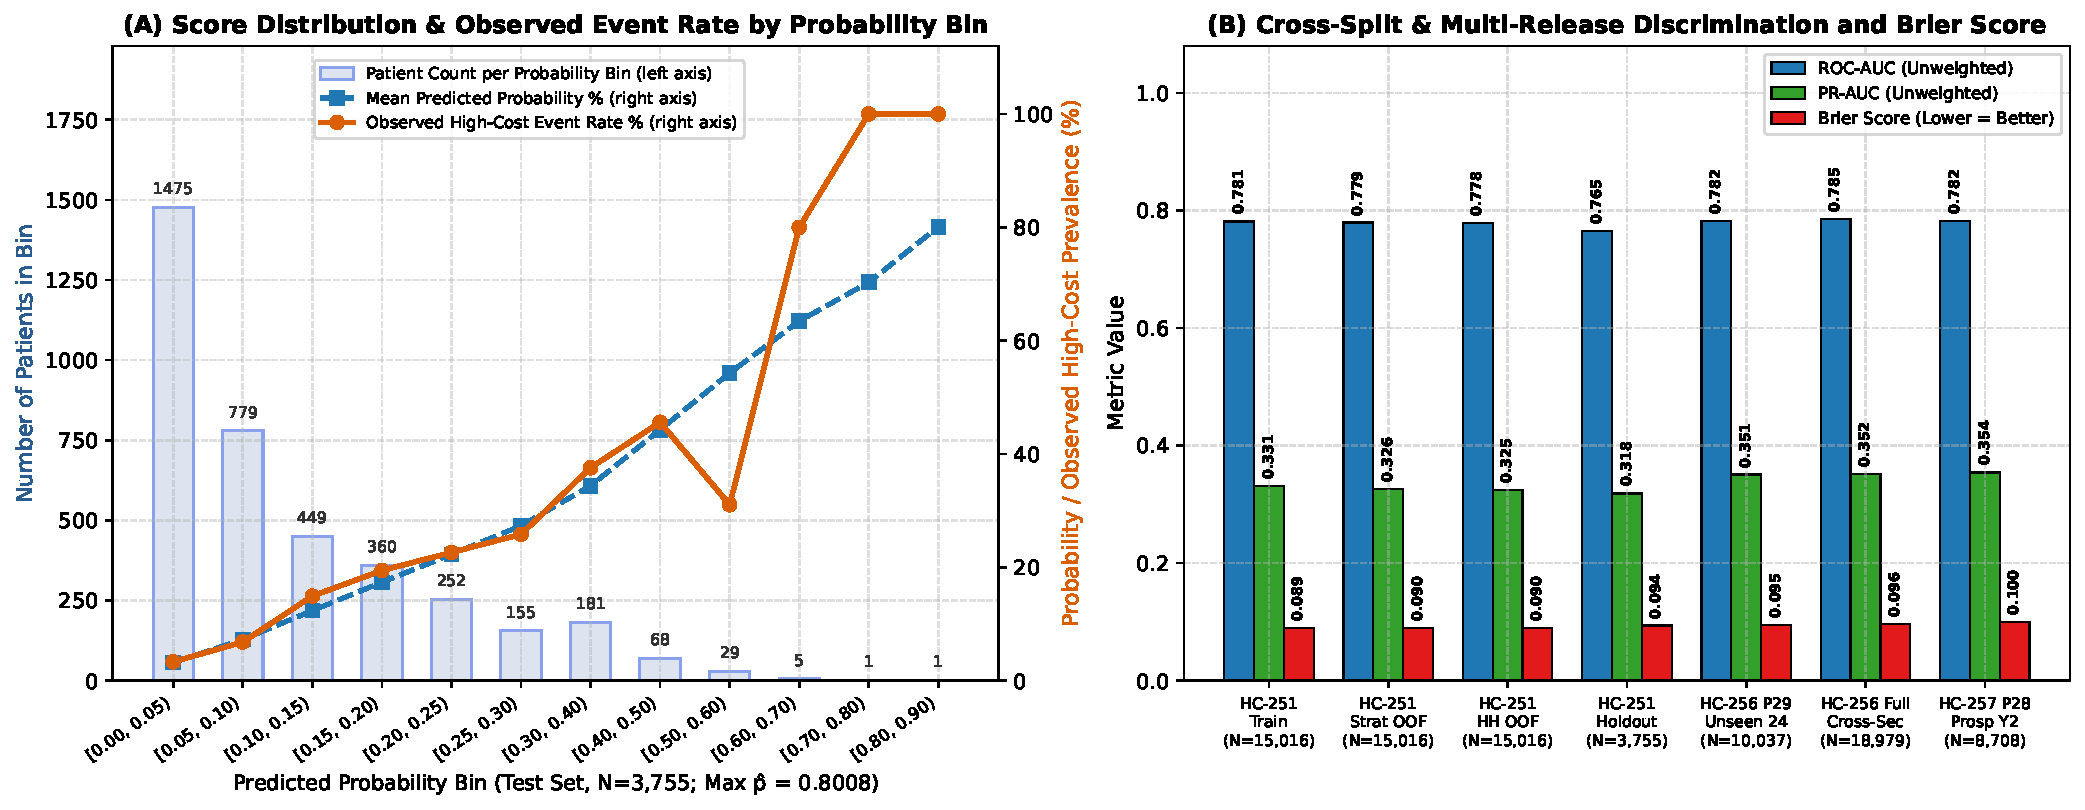
\includegraphics[width=\textwidth]{fig_t5_calibration_and_overfitting_audit.pdf}
\caption{(A) Held-out test cohort probability score distribution and observed vs.\ predicted high-cost event rate by probability bin ($\max \hat{p}_{\text{test}} = 0.8008$) and (B) multi-cohort cross-split and cross-release generalization audit refuting model overfitting.}\label{fig:t5}
\end{figure}

\paragraph{Recommended Three-Tier Operational Decision Framework.}
Rather than restricting clinical deployments to a single binary cutoff, HealthScore exposes the calibrated probability $\hat{p}_i$ alongside three OOF-validated operating regimes tailored to distinct healthcare resource constraints:
\begin{itemize}
    \item \textbf{Tier 1 ($\tau = 0.10$ --- High-Sensitivity Broad Preventive Screening / Max Balanced Accuracy):} Maximizes Balanced Accuracy ($0.7152$ OOF, $0.7122$ Test, $0.7121$ Unseen Panel 29) and captures \textbf{$77.33\%$ of all high-cost patients} ($23.18\%$ precision, $1.93\times$ enrichment, flagging $39.97\%$ unweighted / $33.54\%$ weighted). Appropriate for low-cost automated digital wellness reminders and actuarial tail-risk monitoring where missing a catastrophic patient ($\text{FN}$) is substantially costlier than a false-positive outreach ($\text{FP}$).
    \item \textbf{Tier 2 ($\tau = 0.20$ --- Balanced Care-Management Triage / Validation Primary-Grid F1-Optimal):} Maximizes primary-grid F1 on OOF validation ($\text{OOF F1} = 0.3855$ unweighted, $0.3551$ weighted), achieving \textbf{$30.49\%$ test precision ($2.54\times$ enrichment; $32.69\%$ on unseen Panel 29)}, \textbf{$46.89\%$ test recall ($50.23\%$ OOF, $52.38\%$ Panel 29)}, \textbf{$85.45\%$ specificity}, and \textbf{$\text{F1} = 0.3695$} ($\text{F1} = 0.4026$ on Panel 29), while flagging $18.43\%$ of patients ($13.76\%$ weighted) and \textbf{reducing false positives by $58.28\%$} ($1,153 \to 481$). Programs seeking higher sensitivity within this tier may adopt the intermediate fine-grid cutoff $\tau = 0.15$ ($\text{Test F1} = 0.3742$, $\text{Precision} = 26.71\%$, $\text{Recall} = 62.44\%$).
    \item \textbf{Tier 3 ($\tau = 0.30$ --- High-Specificity Intensive Case Management):} Achieves \textbf{$40.00\%$ test precision ($3.34\times$ enrichment; $42.29\%$ on unseen Panel 29)}, \textbf{$94.83\%$ specificity}, and \textbf{$25.33\%$ recall ($30.29\%$ on Panel 29)} while flagging only the top \textbf{$7.59\%$} of patients ($5.69\%$ weighted) and \textbf{cutting false positives by $85.17\%$} ($1,153 \to 171$). Ideal for capacity-constrained multidisciplinary nurse case management and clinical pharmacist medication reconciliation.
\end{itemize}

\paragraph{Explicit Distinction Between Decision Threshold ($\hat{p} \ge \tau$) and Ranked Cohort Cutoff.}
Evaluating $\hat{p}_i \ge \tau$ applies an individual probability cutoff ($1,501$ flagged at $\tau=0.10$; $692$ at $\tau=0.20$; $285$ at $\tau=0.30$), whereas selecting the top 10\% of individuals ranked by predicted risk ($375$ individuals) is a fixed-capacity decile cutoff (yielding $\approx 42\%$ precision and $\le 35\%$ recall, close to operating between $\tau = 0.25$ [$440$ flagged] and $\tau = 0.30$ [$285$ flagged]).

\subsection{Disclosed Model Weaknesses and Methodological Boundaries}
\begin{enumerate}
    \item \textbf{Dollar-Scale Prediction Limitations:} While tree-based and linear models fit on $\ln(1+y)$ achieve the lowest MAE on the median scale ($\approx \$7,516$), retransforming via $\exp(\hat{y})-1$ severely underpredicts the dollar mean by $72.8\%$ ($\text{Mean Predicted} = \$2,384.13$ vs $\text{Observed} = \$8,764.62$), yielding negative dollar $R^2$ ($-0.0134$). The 11-feature Tweedie GLM ($p=1.5$, log link) directly models un-logged dollars, achieving $R^2 = 0.0798$ (weighted $R^2 = 0.0832$) and tracking the aggregate mean ($\$8,177.92$ vs $\$8,764.62$); however, observed-to-predicted ratios vary across intermediate deciles ($1.766\times$ in Decile 1 to $0.789\times$ in Decile 4).
    \item \textbf{Dominance of the Econometric Persistence Benchmark:} In longitudinal prospective validation on MEPS HC-257 Panel 28 ($N=8,708$), predicting Year 2 spending from Year 1 spending (\texttt{TOTEXPY1}) achieved an $R^2$ of \textbf{$0.1204$} ($\text{MAE} = \$8,625.76$), outperforming static diagnosis-only Tweedie GLM ($R^2 = 0.0652$). Self-reported diagnosis flags alone explain 6--8\% of cost variance; past healthcare utilization remains the dominant predictor of future spending.
    \item \textbf{Subgroup Discrimination Degradation:} On prospective validation (HC-257), high-cost classification discrimination drops from weighted ROC-AUC $0.7807$ on the general population to \textbf{$0.7466$} on the adult SAQ subcohort with self-reported functional limitations, and supplementary fairness audits show poor discrimination in pediatric ($<18$, ROC-AUC $0.40$--$0.49$) and uniformly healthy cohorts.
    \item \textbf{Absence of Decision-Curve Analysis and Standardized Clinical Indices:} Decision-curve analysis (DCA) was not performed, and public MEPS files omit granular 4- and 5-character ICD-10-CM codes required to compute Charlson or Elixhauser comorbidity indices.
\end{enumerate}

% -----------------------------------------------------------------------------
\section{Configurable Loss and Premium Simulation (RQ5)}
% -----------------------------------------------------------------------------

\subsection{Mathematical Formulation and 60-Scenario Sensitivity Grid}
In HealthScore, the output labeled \texttt{premium} is formalized as an exploratory parametric Value-at-Risk (VaR) simulation rather than an actuarially certified commercial insurance premium:
\begin{equation}
X_\alpha = B + (1 + \alpha) G, \quad G \sim \text{Gamma}(k=1.5, \theta=\hat{y}/1.5)
\end{equation}
where $\text{Premium} = \text{Percentile}_{95}(X_\alpha)$, $B \ge 0$ is the configurable base-cost floor in USD (default: $\$500.00$), $E[G] = k\theta = \hat{y}$ is the Tweedie model-predicted expenditure, and $\alpha \ge 0$ is a dimensionless risk-loading parameter (default: $\alpha = 0.0$). For any quantile $q \in (0, 1)$, the theoretical analytical quantile is $Q_{X_\alpha}(q) = B + (1 + \alpha) \cdot \text{Gamma}^{-1}(q; k=1.5, \theta=\hat{y}/1.5)$. We executed a grid sensitivity analysis across 4 base-cost floors ($B \in \{0, 250, 500, 1000\}$), 5 risk-loading levels ($\alpha \in \{0.0, 0.10, 0.25, 0.50, 1.00\}$), and 3 expenditure tiers ($\hat{y} \in \{\$1,500, \$5,000, \$15,000\}$) using Common Random Numbers ($N = 20,000$ draws per scenario; Table~\ref{tab:premium_sensitivity} and Fig.~\ref{fig:premium_sensitivity}). Empirical Monte Carlo simulation tracks closed-form analytical Gamma quantiles within \textbf{$0.68\%$ to $0.71\%$} across all 60 scenarios.

\begin{table}[t]
\centering
\caption{Parametric Value-at-Risk premium simulation sensitivity analysis ($N=20,000$ draws per scenario, Moderate Risk tier $\hat{y} = \$5,000$).}\label{tab:premium_sensitivity}
\resizebox{\textwidth}{!}{%
\begin{tabular}{lcccccccc}
\toprule
\textbf{Tier} & \textbf{Floor $B$} & \textbf{Loading $\alpha$} & \textbf{Sim P5} & \textbf{Sim P50} & \textbf{Sim P95 Premium} & \textbf{Analytical Gamma P95} & \textbf{Error} & \textbf{Premium Uplift} \\
\midrule
Moderate (\$5,000) & \$0.00   & 0.00 & \$727.60   & \$4,007.41 & \textbf{\$13,116.94} & \$13,024.55 & +0.709\% & Baseline (\$0.00) \\
Moderate (\$5,000) & \$0.00   & 0.10 & \$800.36   & \$4,408.15 & \textbf{\$14,428.63} & \$14,327.00 & +0.709\% & +\$1,311.69 (+10.00\%) \\
Moderate (\$5,000) & \$0.00   & 0.25 & \$909.50   & \$5,009.26 & \textbf{\$16,396.17} & \$16,280.68 & +0.709\% & +\$3,279.23 (+25.00\%) \\
Moderate (\$5,000) & \$0.00   & 0.50 & \$1,091.40 & \$6,011.11 & \textbf{\$19,675.41} & \$19,536.82 & +0.709\% & +\$6,558.47 (+50.00\%) \\
Moderate (\$5,000) & \$0.00   & 1.00 & \$1,455.20 & \$8,014.81 & \textbf{\$26,233.88} & \$26,049.09 & +0.709\% & +\$13,116.94 (+100.00\%) \\
Moderate (\$5,000) & \$500.00 & 0.00 & \$1,227.60 & \$4,507.41 & \textbf{\$13,616.94} & \$13,524.55 & +0.683\% & Baseline (\$0.00) \\
Moderate (\$5,000) & \$500.00 & 0.10 & \$1,300.36 & \$4,908.15 & \textbf{\$14,928.63} & \$14,827.00 & +0.685\% & +\$1,311.69 (+9.63\%) \\
Moderate (\$5,000) & \$500.00 & 0.25 & \$1,409.50 & \$5,509.26 & \textbf{\$16,896.17} & \$16,780.68 & +0.688\% & +\$3,279.23 (+24.08\%) \\
Moderate (\$5,000) & \$500.00 & 0.50 & \$1,591.40 & \$6,511.11 & \textbf{\$20,175.41} & \$20,036.82 & +0.692\% & +\$6,558.47 (+48.16\%) \\
Moderate (\$5,000) & \$500.00 & 1.00 & \$1,955.20 & \$8,514.81 & \textbf{\$26,733.88} & \$26,549.09 & +0.696\% & +\$13,116.94 (+96.33\%) \\
\bottomrule
\end{tabular}%
}
\end{table}

\begin{figure}[t]
\centering
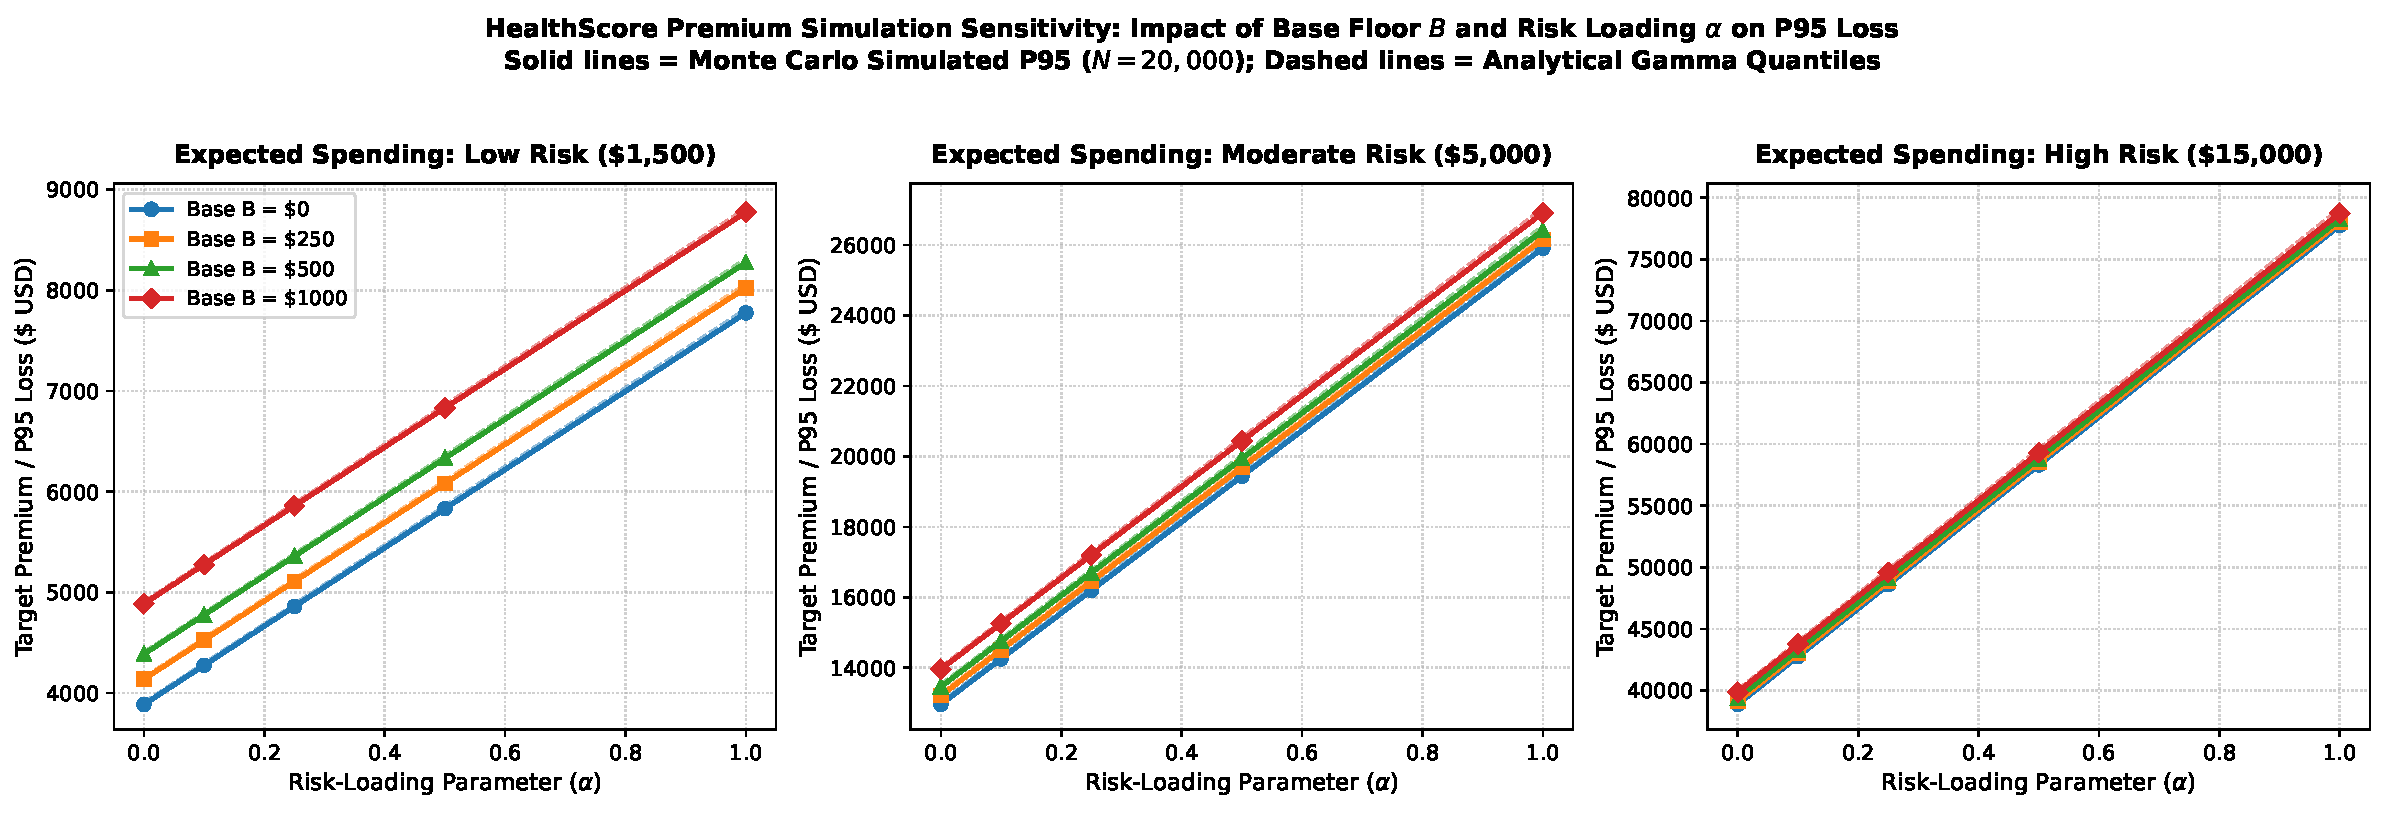
\includegraphics[width=\textwidth]{fig6_premium_sensitivity.pdf}
\caption{HealthScore premium simulation sensitivity: Impact of base floor $B$ and risk loading $\alpha$ on P95 loss across expected spending tiers. Solid lines represent Monte Carlo simulated P95 ($N=20,000$); dashed lines represent analytical Gamma quantiles.}\label{fig:premium_sensitivity}
\end{figure}

% -----------------------------------------------------------------------------
\section{Integrated Discussion: Performance, Practical Use, and Trade-Offs}
% -----------------------------------------------------------------------------

\subsection{Consortium Throughput and Queueing Latency in Healthcare Operations}
For interactive clinical workflows requiring sub-second response times (e.g., bedside vitals recording, prescription creation, or diagnostic scan orders), the consortium network should operate within the linear regime ($\le 200$ write TPS), where committed throughput tracks offered load linearly ($199.9$--$200.2$ TPS) with confirmation latency bounded between $0.03$s and $0.06$s. A major metropolitan health system processing 500,000 clinical encounters per day generates an average load of $\approx 6$--$10$ TPS, peaking at $\approx 50$--$75$ TPS---well within HealthScore's sub-100ms linear window. Under nominal 1,000 TPS stress load, the network sustains $350.1$ TPS ($18.00$s latency) in the historical baseline, $515.8$ TPS ($6.98$s latency) in the 5-worker rerun, and $485.27 \pm 14.60$ TPS ($5.36 \pm 0.22$s latency) in the 8-worker repetitions with zero reported failures among submitted transactions. Because entering the saturation regime incurs multi-second queueing delays ($5.2$--$18.0$s), higher-throughput operation ($470$--$515$ write TPS) is appropriate only for asynchronous, delay-tolerant bulk ingestion protected by client-side rate-limiting queues. At 200 TPS continuous load ($\approx 1.5$ KB/tx), append-only block storage expands by $\approx 1.08$ GB/hour, whereas CouchDB world-state size remains bounded by active patient count $O(N_{\text{patients}})$.

\subsection{Operationalizing Multi-Threshold Clinical Risk Stratification}
Our threshold sensitivity analysis resolves a critical practical challenge in population health management. Operating at $\tau = 0.10$ is optimal only when maximizing Balanced Accuracy ($0.7122$) and sensitivity ($77.33\%$) for low-cost automated outreach, where the $29.98\%$ mathematical volume ceiling bounds precision to $23.18\%$. When clinical care-management teams face staffing or budget constraints, shifting the decision boundary on the exact same calibrated probability output to $\tau = 0.20$ eliminates $58.28\%$ of false positives and raises precision to $30.49\%$ ($32.69\%$ on unseen 2024 Panel 29) while still capturing roughly half of all catastrophic spenders; shifting to $\tau = 0.30$ eliminates $85.17\%$ of false positives and reaches $40.00\%$ precision ($94.83\%$ specificity) for intensive nurse case management.

% -----------------------------------------------------------------------------
\section{Limitations and Threats to Validity}
% -----------------------------------------------------------------------------
\begin{enumerate}
    \item \textbf{Testbed-Specific Benchmark Environment and Absence of Fault-Injection Testing:} All Caliper benchmarks were conducted on a single host (macOS \texttt{arm64}) using Docker bridge networking and single administrative identity \texttt{HospitalOrgAdmin}. Multi-host WAN latency, cross-organization client concurrency, and physical fault-injection experiments (peer crashes, orderer partitions, disk corruption) were not evaluated.
    \item \textbf{Iterative Split Reuse, Unclustered Household Splitting, and Rotating Panel Overlap:} The MEPS HC-251 test partition ($N=3,755$) was reused across benchmark iterations, and row-level splitting in HC-251 shares $2,198$ household \texttt{DUID}s between Train and Test ($72.20\%$ of test rows). Furthermore, MEPS HC-256 ($N=18,979$) shares rotating Panel 28 ($46.24\%$) with HC-251, and HC-257 ($N=8,708$) tracks Panel 28 longitudinally. We mitigated these dependencies by verifying 5-fold \texttt{GroupKFold(groups=DUID)} validation ($\text{ROC-AUC} = 0.7785$) and isolating the $100\%$ unseen HC-256 Panel 29 cohort ($N=10,037$, zero person or household overlap, $\text{ROC-AUC} = 0.7824$).
    \item \textbf{Non-Design-Based Bootstrap Uncertainty:} Reported 95\% confidence intervals derive from non-parametric row-level bootstrap resampling ($B=200$) and do not account for MEPS complex survey clustering (\texttt{VARPSU}) or stratification (\texttt{VARSTR}).
    \item \textbf{Heuristic Clinical Intake Parsing and Absence of ICD-10 Comorbidity Indices:} Runtime feature engineering relies on regex parsing of intake strings where unmentioned conditions default to zero, and public MEPS files omit granular 4- and 5-character ICD-10-CM codes required for Charlson or Elixhauser indices.
    \item \textbf{Direct Dollar Variance Ceiling, Aleatoric Acute Events, and Persistence Dominance:} Static diagnosis flags explain only $\approx 8\%$ of dollar expenditure variance ($R^2 = 0.0798$) and are outperformed by lagged Year-1 spending ($R^2 = 0.1204$). Furthermore, $10.22\%$ of top-decile cases occur in individuals with zero baseline chronic conditions due to stochastic acute events, while $71.79\%$ of individuals with $\ge 3$ chronic clusters do not incur top-decile spending in a given year.
    \item \textbf{No Decision-Curve Analysis, Comparative Privacy Testing, or Actuarial Certification:} Decision-curve analysis (DCA) and comparative encrypted-database privacy benchmarks were outside study scope, and the Monte Carlo VaR premium simulation ($X_\alpha = B + (1+\alpha)G$) is strictly an exploratory technical demonstration uncertified for commercial underwriting or statutory solvency.
\end{enumerate}

% -----------------------------------------------------------------------------
\section{Conclusion}
% -----------------------------------------------------------------------------
This paper presented an empirical performance, statistical, and systems evaluation of \textbf{HealthScore}, uniting a 5-organization permissioned Hyperledger Fabric blockchain consortium with an off-chain ACG-inspired multi-disease risk engine and an exploratory Value-at-Risk premium simulation. Our Caliper benchmarks demonstrate $199.9$--$200.2$ write TPS with sub-$100$ms latency in the linear regime, $350.1$--$515.8$ write TPS under stress saturation with zero reported transaction failures among submitted proposals, and $500.3$--$500.6$ read TPS ($\le 0.01$s displayed average latency), while highlighting the $\approx 20$--$25$ req/s single-worker off-chain ML inference boundary.

Across $46,458$ MEPS records, controlled 17-scenario feature ablations confirm that custom ACG-inspired chronic-condition clusters provide the primary predictive lift over demographics ($R^2 = 0.0395 \to 0.0771$, weighted BSS $+0.0506 \to +0.1025$). Our deployed 11-feature Observable Logistic Regression classifier achieves ROC-AUC $0.7654$, PR-AUC $0.3184$, and weighted BSS $+0.1025$ on the held-out test set and ROC-AUC $0.7824$ on the $100\%$ unseen 2024 Panel 29 cohort ($N=10,037$). Through a rigorous 12-threshold sensitivity analysis ($\tau \in [0.05, 0.90]$) validated via leak-free 5-fold OOF cross-validation, we proved that the $23.18\%$ precision at $\tau = 0.10$ ($77.33\%$ recall) is governed by the $29.98\%$ mathematical volume ceiling when screening $39.97\%$ of a skewed population rather than overfitting, and established validated operational tiers at $\tau = 0.20$ ($30.49\%$ test precision, $32.69\%$ Panel 29 precision, $58.28\%$ fewer false positives) and $\tau = 0.30$ ($40.00\%$ test precision, $94.83\%$ specificity, $85.17\%$ fewer false positives) to support resource-aware clinical triage.

% -----------------------------------------------------------------------------
% Bibliography
% -----------------------------------------------------------------------------
\bibliographystyle{splncs04}
\bibliography{references}

\end{document}
